\chapter{Determining $H_0$ with Bayesian hyper-parameters}
\label{chapter-h0}

\section{Introduction}
\label{chapter-h0:introduction}

Pinning down the Hubble constant $H_0$ is crucial for the understanding of the standard model of cosmology. It sets the scale for all cosmological times and distances and it allows to tackle cosmological parameters, breaking degeneracies among them (e.g., the equation of state for dark energy and the mass of neutrinos). The expansion rate of the universe can either be directly measured or inferred for a given cosmological model through cosmological probes such as the cosmic microwave background (CMB). Although accurate direct measurements of the Hubble constant have proven to be difficult (e.g., control of systematic errors, relatively small data sets, fully consistency of different methods for measuring distances), significant progress has been achieved  
over the past decades \cite{Freedman1996,Freedman:2010xv}. The \textit{Hubble Space Telescope (HST)} Key Project made possible to measure $H_0$ with an accuracy of $10\%$ by significantly improving the control of systematic errors \cite{Freedman2001}.  More recently, in the \textit{HST} Cycle $15$, the \textit{Supernovae and $H_0$ for the Equation of State (SHOES)} project has reported measurements of $H_0$ accurate to $4.7\%$ ($74.2 \pm 3.6 \, \km\, \second^{-1}\, \Mpc^{-1}$) \cite{Riess:2009pu}, then to $3.3\%$ ($73.8 \pm 2.4 \, \km\, \second^{-1}\, \Mpc^{-1}$) \cite{Riess:2011yx} and very recently to $2.4\%$ ($73.24 \pm 1.74 \, \km\, \second^{-1}\, \Mpc^{-1}$) \cite{Riess:2016jrr}. This remarkable progress has been achieved thanks to both an enlarged sample of SN Ia having a Cepheid calibrated distance, a reduction in the systematic uncertainty of the maser distance to $\NGC$, an increase of infrared observations of Cepheid variables in the Large Magellanic Cloud (LMC).  

The 2015 release in temperature, polarization and lensing measurements of the CMB by the \textit{Planck} satellite leads to a present expansion rate of the universe given by $H_0 = 67.81 \pm 0.92 \, \km \, \second^{-1}\, \Mpc^{-1}$ for the base six-parameter $\Lambda$CDM model \cite{Ade:2015xua}. As it is known, the derived estimation of $H_0$ from CMB experiments provide indirect and highly model-dependent values of the current expansion rate of the universe (requiring e.g., assumptions about the nature of dark energy, properties of neutrinos, theory of gravity) and therefore do not substitute a direct measurement in the local universe. Moreover, indirect determinations (in a Bayesian approach) rely on prior probability distributions for the cosmological parameters which might have an impact on the results.

The \textit{Planck} Collaboration used a ``conservative'' prior on the Hubble constant ($H_0=70.6\pm3.3\, \km\, \second^{-1}\, \Mpc^{-1}$) derived from a reanalysis of the Cepheid data used in \cite{Riess:2011yx}, done by G. Efstathiou in \cite{Efstathiou:2013via}: in this reanalysis, a different rejection algorithm was used (with respect to that in \cite{Riess:2011yx}) for outliers in the Cepheid period-luminosity relation (the so-called Leavitt Law); in addition, \cite{Efstathiou:2013via} used the revised geometric maser distance to $\NGC$ of \cite{Humphreys:2013eja}. Although consistent with the \textit{Planck} TT estimate at the $1\, \sigma$ level, this determination of $H_0$ assumes that there is no metallicity dependence in the Leavitt Law. Furthermore, it discards data (i) from both Large Magellanic Cloud (LMC) and Milky Way (MW) Cepheid variables (ii) from the sample of Cepheid variables in \cite{Riess:2011yx} using an upper period cut of $60$ days.\footnote{In \cite{Efstathiou:2013via} G. Efstathiou also shows results utilizing the rejection algorithm for outliers used in \cite{Riess:2011yx}, but with the revised geometric maser distance to $\NGC$ \cite{Humphreys:2013eja} which is about $4\%$ higher than that adopted by \cite{Riess:2011yx} in their analysis. Note that in \cite{Riess:2011yx} (see their page 13) the authors provided a recalibration of $H_0$ for each increase of $1\%$ in the distance to $\NGC$ : according to this recalibration and the revised geometric maser distance their measurement would be driven downwards from $H_0 = 74.8\, \km \, \second^{-1}\, \Mpc^{-1}$ to $H_0 \approx 73.8 \, \km \, \second^{-1}\, \Mpc^{-1}$ which is higher than all the reported values in table A1 of \cite{Efstathiou:2013via} for the R11 rejection algorithm.}

As discussed in \cite{Freedman:2010xv}, the sensitivity to metallicity of the Leavitt Law is still an open question. In fact, due to changes in the atmospheric metal abundance, a metallicity dependence in the Cepheid period-luminosity is expected. Discarding data involves somehow arbitrary choices (e.g., chauvenet's criterion, period cut, threshold T in \cite{Efstathiou:2013via}) and might hinder our understanding of the physical basis behind the incompatibility of data sets (if any) \cite{Press:1996fw}. Therefore, neither no metallicity dependence in Leavitt Law nor disregarding data seem to be very conservative assumptions. 

Once systematics are under control (like the presence of unmodeled systematic errors or biases in the outlier rejection algorithm for Cepheid variables), a reliable estimate of $H_0$ is very important also on theoretical grounds. Confirmation of significant discrepancies between direct and indirect estimates of $H_0$ would suggest evidence of new physics. Discrepancies could arise if the local gravitational potential at the position of the observer is not consistently taken into account when measuring the Hubble constant. Nevertheless, an unlikely fluctuation would be required to explain an offset as big as $2.4\,\sigma$ \cite{Marra2013a}. Second-order corrections to the background distance-redshift relation could bias estimations of the Hubble constant derived from CMB \cite{Clarkson:2014pda}. However, it was shown in \cite{Bonvin:2015uha} that those corrections are already taken into account in current CMB analyses.           

It is clear from \cite{Efstathiou:2013via} that the statistical analysis done when measuring $H_0$ plays a part in the final result (for instance, through the outlier rejection algorithm, data sets included, anchors distances included, the period cut on the sample of Cepheid variables, the prior on the parameters of the Period-Luminosity relation). Given the relevance of the Hubble constant for our understanding of the universe, it is necessary to confirm previous results and prove them robust against different statistical approaches.

The goal of this project is to determine the Hubble constant $H_0$ by using Bayesian hyper-parameters to reanalyse the Cepheid data set used in both \cite{Riess:2011yx} and \cite{Riess:2016jrr}. In Section \ref{chapter-h0:notation-and-method} we explain both our notation and the statistical method employed. We then apply the method to different data sets and determine $H_0$ in Section \ref{chapter-h0:Application}. We conclude and discuss our results in Section \ref{chapter-h0:Summary}. 

\section{Notation and formalism}
\label{chapter-h0:notation-and-method}

\subsection{Distances and standard candles}

Astrophysical objects with a known luminosity -- the so-called standard candles-- are used to probe the expansion rate of the universe. In particular, measuring redshifts and apparent luminosities for supernovae type Ia (SNe Ia) one can establish an empirical redshift-distance relation for these objects. In order to estimate distances to SNe Ia one uses the luminosity distance
\begin{equation}
d_L \equiv \left(\frac{L}{4\pi l} \right)^{1/2} \, , \label{Eq:luminosity-distance-obs}
\end{equation}
where $L$ and $l$ are the absolute luminosity and the apparent luminosity, respectively. For historical reasons the apparent bolometric luminosity $l$ is defined so that 
\begin{equation}\label{Eq:apparent-luminosity}
l = 10^{-2m/5}\times 2.52 \times 10^{-5}\, \mathrm{erg/ cm^2}\, \second
\end{equation}
where $m$ is the apparent bolometric magnitude \cite{Weinberg:1972kfs}. Similarly, one can define the absolute bolometric magnitude $M$ as the apparent bolometric magnitude a source would have at a distance 10 $\mathrm{pc}$
\begin{equation}\label{Eq:absolute-luminosity}
L = 10^{-2M/5} \times 3.02 \times 10^{35}\, \mathrm{erg/}\second.
\end{equation}
Combining equations \eqref{Eq:luminosity-distance-obs}-\eqref{Eq:absolute-luminosity} it is possible to express the luminosity distance in terms of the distance modulus $m-M$:
\begin{equation}
\mu_0 \equiv m - M = 5 \log_{10} \left(\frac{d_L}{1 \mathrm{Mpc}} \right) + 25 \, . \label{Eq:distance-modulus}
\end{equation}

One can also estimate the luminosity distance $d_L$ of a light source with redshift $z$ within the context of General Relativity. Assuming a flat FLRW metric, one can compute the luminosity distance  
\begin{equation}\label{Eq:luminosity-distance-the}
d_L(z) = (1+z) c \int_0^z \frac{dz'}{H(z')} \, 
\end{equation}
where $c$ is the speed of light and $H(z)$ is the Hubble function. Since nowadays the empirical curve for $d_L(z)$ is reasonably well known for relatively small redshift, the Hubble function may then be usefully expressed as a power series in Eq. \eqref{Eq:luminosity-distance-the} leading to
\begin{equation}\label{Eq:luminosity-distance-the-small-z}
d_L(z) \equiv \frac{cz}{H_0}  ( 1+\delta(z)) \approx \frac{cz}{H_0} \left\{ 1 + \frac{1}{2} [1-q_0] z - \frac{1}{6} [1-q_0 - 3 q_0^2 + j_0] z^2 + O(z^3) \right\}
\end{equation} 
where $H_0$ is the Hubble constant, $q_0$ is the present acceleration parameter, $j_0$ the present prior deceleration parameter, and $\delta(z)$ defines a function that vanishes as $z\rightarrow 0$ and can be approximately expressed as a series expansion in redshift starting with a term linear in $z$.

Having both an empirical curve and a theoretical estimation of $d_L(z)$ for a given set of astrophysical objects we can then try to find the parameters which fit the data the best. Equating Eqs. \eqref{Eq:distance-modulus} and \eqref{Eq:luminosity-distance-the-small-z} we obtain that
\begin{equation}\label{Eq:av-definition}
5 \log_{10} ( c z ( 1+\delta(z) )) - m_X = 5 \log_{10} H_0 - M_X - 25 \equiv 5 a_X \, ,
\end{equation}
where $X$ denotes the use of wavelength band $X$ (e.g., $U$ for ultraviolet, $B$ for blue, and $V$ for visual) and $a_X$ is a constant which defines the intercept of the $\log_{10} cz - 0.2\, m_X$ relation. Defining $\delta(z)$ through $q_0 = -0.55$ and $j_0 = 1$ \cite{Riess:2006fw}, Riess et al. \cite{Riess:2011yx} used the $V$ wavelength band Hubble diagram for 153 nearby SN-Ia in the red shift range $0.023 < z < 0.1$ (a conservative lower limit in red shift imposed to avoid the possibility of a local, coherent flow biasing the results)
to measure the intercept $a_V = 0.697 \pm 0.00201$. Using the Hubble diagram for $217$ $\SNe$ in the red shift range $0.023 < z < 0.15$, Riess et al. \cite{Riess:2016jrr} found $a_B = 0.71273 \pm 0.00176$.

From Eqs. \eqref{Eq:distance-modulus} and \eqref{Eq:av-definition} one can easily express the apparent magnitude $m_X^{\SNe}$ of a SNe Ia in terms of its distance modulus $\mu_0$, the Hubble constant $H_0$, and the intercept $a_X$ as
\begin{equation}
m_X^{\SNe} =  5 \log_{10} H_0 + \mu_0 - 5 a_X - 25 \, . \label{Eq:apparent-magnitude-H0}
\end{equation}
At this point (having measured $a_X$) we are again in a position where we can try to find the parameters $H_0$ and $\mu_0$ which adjust the best the observed $m^{\SNe}_X$. Cepheid variables -- another type of standard candle -- are stars whose apparent luminosity is observed to vary more or less regularly with time. There exist a few known galaxies ($19$ up to date \cite{Riess:2016jrr}) which simultaneously host both SNe Ia and Cepheid variables providing thus the means to measure the distance parameter $\mu_{0,i}$ for the $i\mathrm{th}$ SN Ia through the Leavitt Law \cite{1912HarCi.173....1L}. According to the Leavitt Law there is a relation between period and luminosity of Cepheids: in the $i\mathrm{th}$ galaxy, the pulsation equation for the $j\mathrm{th}$ Cepheid star with apparent magnitude $m^{\Cepheid}_{X,i,j}$ (in the passband $X$) and period $P_{i,j}$ leads to a relation 
\begin{equation}\label{Eq:P-L-equation}
m^{\Cepheid}_{X,i,j} = \mu_{0,i} + M^{\Cepheid}_X + b_X (\log P_{i,j}-1) + Z_X \Delta \log[O/H]_{i,j},
\end{equation}
where $Z_X$ is the metallicity parameter, $b_X$ is the slope of the period-luminosity relation, and $M^{\Cepheid}_X$ is the Cepheid zero point. In principle, a simultaneous fit of Eqs. \eqref{Eq:apparent-magnitude-H0} and \eqref{Eq:P-L-equation} to observed $\SNe$ and Cepheid variables magnitudes would provide constraints for the expansion rate of the universe. 

Constraints for the parameters of the period-luminosity relation \eqref{Eq:P-L-equation} can be improved by adding to the fit galaxies containing Cepheid stars and for which a direct measurement of their distance (or the derived distance modulus $\mu_0$) is known. This is the case for the megamaser system $\NGC$, LMC, and M31. Although the sample of MW Cepheid variables with parallax measurements is relatively small ($15$ up to date \cite{Riess:2016jrr}) and mostly dominated by Cepheid stars with period $P<10$ days, their inclusion helps to further constrain parameters in the period-luminosity relation. Therefore, the inclusion of any of these anchor distances in a simultaneous fit to Eqs. \eqref{Eq:apparent-magnitude-H0}-\eqref{Eq:P-L-equation} helps to improve constraints on the distance parameters $\mu_{0,i}$ for the SNe Ia hosts and hence the Hubble constant $H_0$. 

\subsection{Hyper-parameters}

Astrophysical observations are difficult, and it is not easy to estimate and include the associated errors and uncertainties correctly. Often the data sets show outliers with error bars that are much smaller than the standard deviation from the expected fit, for reasons that are not well understood or difficult to quantify. An analysis needs to deal with such outliers, typically by removing them based on some rejection rule.
As discussed in \cite{Riess:2009pu,Riess:2011yx,Efstathiou:2013via}, the rejection of outliers on the Cepheid period-luminosity relation has a non-negligible effect on the determination of the expansion rate of the universe. One can argue that an outlier rejection criterion: i) involves arbitrary choices (e.g., Chauvenet's criterion, period cut) which might bias the results ii) rejects data, thus increasing error bars and hindering a better understanding of the data sets \cite{Press:1996fw}. The hyper-parameters (HPs, hereafter) method offers a Bayesian alternative to {\em{ad hoc}} selection of data points, avoiding problems associated with using incompatible data points \cite{Lahav:1999hu}. Instead of adopting an a priori rejection criterion  (galaxy-by-galaxy basis as in \cite{Riess:2009pu,Riess:2011yx} or from a global fit as in \cite{Efstathiou:2013via}), in this work we analyse {\em all} the available measurements with Bayesian HPs. The latter effectively allow for relative weights in the Cepheid variables, determined on the basis of how good their simultaneous fit to the model is. 

HPs allow to check for unrecognised systematic effects by introducing a rescaling of the error bar of data point $i$, $\sigma_i \rightarrow \sigma_i/\sqrt{\alpha_i}$. Here $\alpha_i$ is a HP associated with the data point $i$ \cite{Lahav:1999hu}.
In order to explain how HPs work, we start by assuming a Gaussian likelihood for the datum $D_i$,
\begin{equation}\label{Eq:Gaussian-likelihood}
P_G(D_i|\vec{w}) = \tilde{N}_i \, \frac{\exp(-\chi^2_i(\vec{w})/2)}{\sqrt{2\pi}},
\end{equation}
where $\chi^2_i$ and the normalisation constant $\tilde{N}_i$ are given by
\begin{equation}\label{Eq:chi2} %\label{Eq:normalization-Gaussian-likelihood}
\chi^2_i \equiv \frac{\left( x_{\obs,i} - x_{\pred,i}(\vec{w}) \right)^2}{\sigma_i^2} \, , \quad
\tilde{N}_i = 1/\sqrt{\sigma_i^2} \, .
\end{equation}
Here for each measurement $x_{\obs,i}$ there is a corresponding error $\sigma_i$ and a prediction $x_{\pred,i}(\vec{w})$, ($\vec{w}$ being the parameters of a given model). Suppose that some errors have been wrongly estimated due to unrecognised (or underestimated) systematic effects and use hyper-parameters  \cite{Lahav:1999hu} to control the relative weight of the data points in the likelihood. For each measurement {$i$} we introduce a HP to rescale $\sigma_i$ as mentioned above. In that case the Gaussian likelihood becomes \cite{Lahav:1999hu}
\begin{equation}\label{Eq:HP-Gaussian-likelihood}
P(D_i|\vec{w},\alpha_i) = \tilde{N}_i \, \alpha_i^{1/2}\, \frac{\exp(-\alpha_i \chi^2_i(\vec{w})/2)}{\sqrt{2\pi}}.
\end{equation}

However, in general we do not know what value of $\alpha_i$ is correct. In order to circumvent this problem, 
we follow a Bayesian approach, introducing the $\alpha_i$ as nuisance parameters and marginalising over them. Given a set of data points $ \lbrace D_i \rbrace$, we can write the probability for the parameters $\vec{w}$  as
\begin{equation}\label{Eq:probability-of-w}
P(\vec{w}|\lbrace D_i \rbrace) = \int \dots \int P(\vec{w},\lbrace \alpha_i \rbrace|\lbrace D_i \rbrace)\, d\alpha_1 \dots d\alpha_N,
\end{equation}
where $N$ is the total number of measurements. Bayes' theorem allows us to write 
\begin{equation}\label{Eq:probability-of-w-alphas-1}
P(\vec{w},\lbrace \alpha_i \rbrace|\lbrace D_i \rbrace) = \frac{P(\lbrace D_i \rbrace|\vec{w},\lbrace \alpha_i \rbrace)\, P(\vec{w},\lbrace \alpha_i \rbrace)}{P(D_1,\dots,D_N)}
\end{equation}
and 
\begin{equation}\label{Eq:probability-of-w-alphas-2}
P(\vec{w},\lbrace \alpha_i \rbrace) = P(\vec{w}|\lbrace \alpha_i \rbrace)\, P(\lbrace \alpha_i \rbrace).
\end{equation}
As in \cite{Lahav:1999hu} we assume:
\begin{subequations}\label{Eq:assumptions}
\begin{align}
\label{Eq:assumptions:1}
P(\lbrace D_i \rbrace|\vec{w},\lbrace \alpha_i \rbrace) & = P(D_1|\vec{w},\alpha_1)\dots P(D_N|\vec{w},\alpha_N),
\\
\label{Eq:assumptions:2}
P(\vec{w}|\lbrace \alpha_i\rbrace) & = \mathrm{constant},
\\
\label{Eq:assumptions:3}
P(\lbrace \alpha_i \rbrace) & = P(\alpha_1)\dots P(\alpha_N).
\end{align}
\end{subequations}

Thus far the formalism is fairly general and it contains two unspecified functions: probability distributions for both data points and HPs. In this work we will assume uniform priors for HPs ($P(\alpha_i)=1$) and that errors never become smaller than their reported value ($\alpha_i \in [0,1]$).\footnote{We have examined the more general case of an improper Jeffrey's prior (allowing decreasing as well as increasing error bars). This works well when many data points are associated to the same HP so that the $\chi^2$ never vanishes. But when each data point has its own associated HP then the model curve can pass through that data point so that $\chi^2_i=0$. In this case the likelihood grows without bounds as $\alpha_i\rightarrow 0$, in other words the HP-marginalised likelihood is singular when at least one of the points has $\chi^2=0$ as can also be seen from Eq. (16) in \cite{Lahav:1999hu}.} A low posterior value of the HP indicates that the point has less weight within the fit. This may indicate the presence of systematic effects or the requirement for better modelling. With these assumptions Eq.~\eqref{Eq:probability-of-w} now becomes:

\begin{equation}\label{Eq:probability-of-w-2}
P(\vec{w},\lbrace D_i \rbrace) = \frac{P(D_1|\vec{w})\dots P(D_N|\vec{w})}{P(D_1,\dots,D_N)},
\end{equation}
where 
\begin{equation}\label{Eq:probability-of-w-2b}
P(D_i|\vec{w}) \equiv \int_0^1 P(D_i|\vec{w},\alpha_i)\, d\alpha_i.
\end{equation}

The integral in Eq. \eqref{Eq:probability-of-w-2b} can be explicitly evaluated for the Gaussian HP likelihood (\ref{Eq:HP-Gaussian-likelihood}), it gives, for each data point,
\begin{eqnarray}\label{Eq:hyper-likelihood}
P(D_i|\vec{w}\,) = \tilde{N}_i \, \left(\frac{ \mathrm{Erf}\left( \frac{\chi_i(\vec{w})}{\sqrt{2}} \right)  -\sqrt{\frac{2}\pi} \chi_i(\vec{w}) \exp(-\chi^2_i(\vec{w})/2)}{ \chi^3_i(\vec{w})} \right).
\end{eqnarray}
We can now rewrite Eq. \eqref{Eq:probability-of-w-2} as
\begin{equation}\label{Eq:probability-of-w-2c}
\ln P(\vec{w},\lbrace D_i \rbrace) = \sum_i \ln \tilde{N}_i + \ln \tilde{\chi}^2_i, 
\end{equation} 
where constant terms have been omitted and where
\begin{equation}\label{Eq:hyper-chi2}
\tilde{\chi}^2_i(\chi^2_i(\vec{w})) \equiv \frac{ \mathrm{Erf}\left( \frac{\chi_i(\vec{w})}{\sqrt{2}} \right)  -\sqrt{\frac{2}\pi} \chi_i(\vec{w}) \exp(-\chi^2_i(\vec{w})/2)}{ \chi^3_i(\vec{w})}.
\end{equation}

One can easily obtain the most likely value for each HP by maximizing \eqref{Eq:HP-Gaussian-likelihood} w.r.t HPs at a given set of best fit parameters $\vec{w}$. We find that for each data point the effective HP is given by:
\begin{subequations}\label{Eq:effective-HPs}
\begin{align}
\label{Eq:effective-HP-1}
\alpha^{\eff}_i & = 1,\quad \mathrm{if} \quad \chi^2_i\leq1
\\
\label{Eq:effective-HP-2}
\alpha^{\eff}_i & = \frac{1}{\chi^2_i},\quad \mathrm{if} \quad \chi^2_i> 1.
\end{align}
\end{subequations}
We will now apply HPs to combine Cepheid variable measurements and determine the current expansion rate of the universe. We explore the parameter space $\vec{w}$ with the help of a Markov Chain Monte Carlo (MCMC) approach using flat priors if not specified differently.

\begin{figure}[hbtp]
\centering
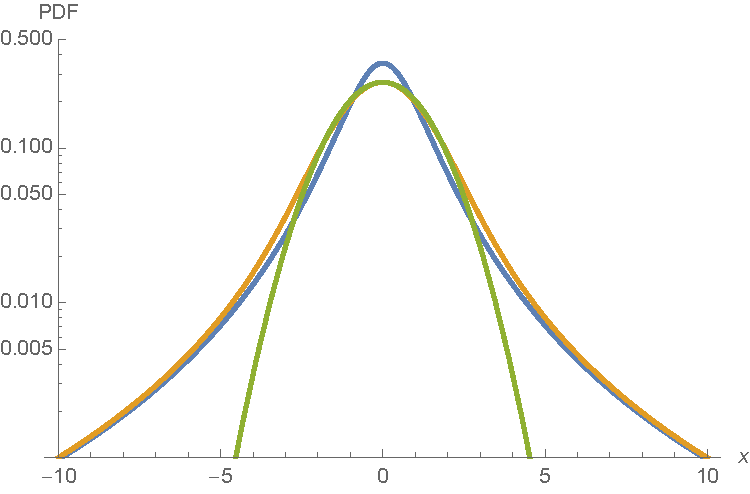
\includegraphics[scale=1]{figures/chapter-h0/hyperparam_like.pdf}
\caption{The hyperparameter-marginalized probability distribution function (pdf) of Eq.\ (\ref{Eq:hyper-likelihood}) in yellow. Close to the origin, $x=0$, it is similar to a Gaussian pdf with $\sigma = (5/2)^{1/3}$ (green), except that its amplitude at the peak is 10.5\% lower than a normalised Gaussian. Asymptotically for $|x|\rightarrow\infty$ it decreases as $1/x^3$ and looks like a student's t distribution with 2 degrees of freedom (blue), but the latter is narrower at small $x$.}
\end{figure}

\section{Applying hyper-parameters}
\label{chapter-h0:Application}

In this section we will apply HPs to determine the Hubble constant. First, we will illustrate how the method works by fitting the period-luminosity relation of Cepheid variables in the LMC, the MW, and the megamaser system $\NGC$. This will allow us to compare with results in \cite{Efstathiou:2013via}. Then in Subsection \ref{Subsection:combining-anchors} we determine $H_0$ with the Cepheid sample and SNe hosts in \cite{Riess:2011yx} (hereafter, R11). When this work was about to finish a new enlarged, improved sample of Cepheid variables and SNe hosts came out \cite{Riess:2016jrr} (hereafter, R16); we determine the expansion rate of the universe with this data set in Subsection \ref{Subsection:combining-anchors-R16}.  

\subsection{The LMC Cepheid variables}
\label{Subsection:LMC}

We start out our analysis by applying HPs to the set of 
53 LMC Cepheid variables with $H$-band magnitudes, $m_H$, listed in Table 3 of  \cite{2004AJ:128.2239P} and $V$, $I$ band magnitudes, $m_V$, $m_I$, listed in Table 4 of \cite{2002ApJS:142:71S}. Following \cite{Riess:2016jrr}, we rely primarily on (near-infrared) NIR ``Wesenheit reddening-free'' magnitudes, defined as 
\begin{equation}\label{Eq:Wesenheit-reddening-free}
m_{W,i} = m_{H,i} - R\, (m_{V,i} - m_{I,i}),
\end{equation}
where $R$ is a constant defining the reddening law; In Subsections \ref{Subsection:LMC}-\ref{Subsection:combining-anchors}, where R11 data set is used, we set $R=0.410$ as G. Efstathiou did \cite{Efstathiou:2013via}; When utilising R16 data set, we analyse the sensitivity of $H_0$ to variations in $R$. For the purpose of comparing with \cite{Efstathiou:2013via} we neglect for now metallicity dependence and fit the data with a period-luminosity relation
\begin{equation}\label{Eq:P-L-LMC}
m^P_W = A + b_W (\log P - 1)
\end{equation}
where $A = \mu_{0,\LMC} + M_W$ in notation of Eq. \eqref{Eq:P-L-equation} and $P$ is the period.\footnote{We have dropped the label '$\Cepheid$' in the magnitudes for sake of simplicity.} In order to apply HPs we define 
\begin{equation}\label{Eq:chi2-LMC}
\chi^{2,\LMC}_{i} = \frac{(m_{W,i} - m^P_{W})^2}{\sigma_i^2 + \sigma^{2,\LMC}_{\intt}},
\end{equation}
where $\sigma_i$ is the observational error on $m_{W,i}$ and $\sigma_{\intt}^{\LMC}$ is what is referred to as `internal scatter' in \cite{Efstathiou:2013via}. The internal scatter is a common additional dispersion of the data points that is independent of the measurement error and due to variations in the physical mechanism behind the period-luminosity relation. As we do not know the origin and magnitude of the internal scatter precisely, we add it as an additional random variable and marginalise over it.\footnote{Note that in R16 data set this intrinsic dispersion is already included in the total statistical uncertainty reported in their table 4 \cite{Riess:2016jrr}. Consequently, when analysing R16 data set we do not include an additional $\sigma_{\intt}$.} More precisely, we sample in $\log \sigma_{\intt}$ with a flat prior $\ln \sigma_{\intt} \in [-3,-0.7]$.
Maximizing  
\begin{equation}
\label{Eq:likelihood-HP-LMC}
\ln P^{\LMC}(A,b_W,\lbrace D_i \rbrace) = \sum_{i} \ln \tilde{\chi}_i^{2}(\chi^{2,\LMC}_{i}) + \ln \tilde{N}^{\LMC}_{i},
\end{equation}
where 
\begin{equation}
\label{Eq:normalization-LMC}
\tilde{N}^{\LMC}_i = \frac{1}{\sqrt{\sigma_i^2 +\sigma^{2,\LMC}_{\intt}}},
\end{equation}
we find the best-fitting parameters of the period-luminosity relation \eqref{Eq:P-L-LMC}. Table \ref{Table:LMC-fits} shows results for different period cuts. Figure \ref{Fig:LMC-Cepheid-variables-fit-c} shows period-luminosity relation for the LMC Cepheid variables and the best fit of cases (c) and (d) in Table \ref{Table:LMC-fits}. We also show in Fig.\ \ref{fig:sigmaint} the posterior probability distribution function (pdf) of $\sigma_{\intt}$ for the fits (c) and (d) of Table \ref{Table:LMC-fits}.

\begin{table}[tbp]
\centering
\begin{tabular}{@{}ccccc}
\hline
\multicolumn{5}{c}{LMC Cepheid variables} \\
\hline
Fit & $A$ & $b_W$ & $\sigma_{\intt}^{\LMC}$ & Period cut \\
\hline
 a & $12.570\,(0.035)$ & $-3.32\,(0.10)$ & $0.06$ & $10<P<60$ \\
  
 b & $12.562\,(0.016)$&$-3.30\,(0.05)$ & $0.06$ & $P<60$ \\

 c & $12.562\,(0.016)$& $-3.31\,(0.05)$& $0.06$ & $P<205$ \\

 d & $12.555\,(0.019)$& $-3.24\,(0.06)$& $0.12$ & $P<205$ \\
\hline
\end{tabular}
\caption{\label{Table:LMC-fits} Mean value and standard deviation (in brackets) for the parameters in the period-luminosity relation. Fits a, b, and c use HPs whereas fit d is a standard $\chi^2$ minimization as done in \cite{Efstathiou:2013via}.}
\end{table}


\begin{figure}[tbp]
\centering % \begin{center}/\end{center} takes some additional vertical space
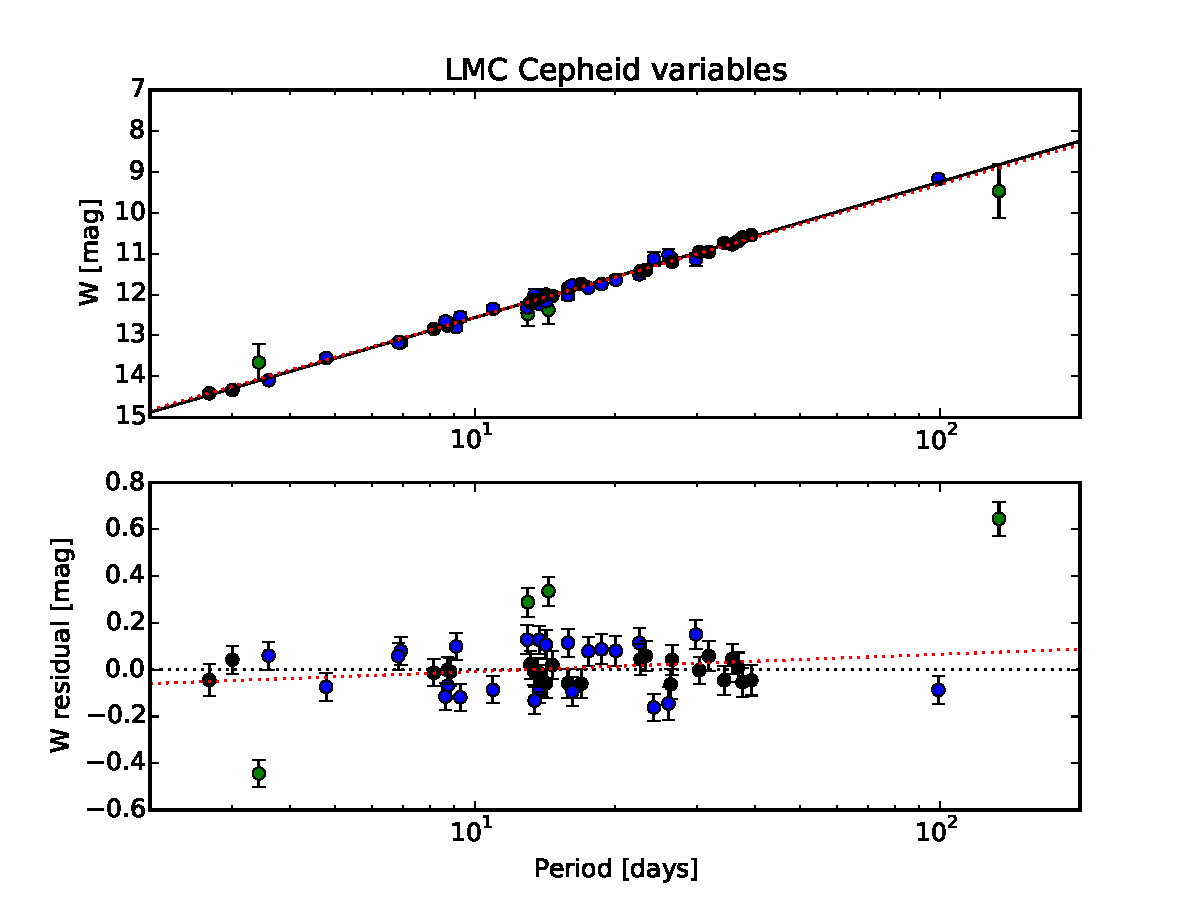
\includegraphics[scale=0.75]{figures/chapter-h0/effective_HP_cepheids_LMC.pdf} 
\caption{Period-luminosity relation for the LMC Cepheid variables. The upper panel shows the best fit of both the case (c) (solid black line) and case (d) (red dotted line) in Table \ref{Table:LMC-fits}. Error bars have been rescaled with corresponding effective HPs which are colour-coded as follows: black if $\alpha_{\eff} = 1$, blue if $10^{-1}\leq \alpha_{\eff} < 1$, green if $10^{-2}\leq \alpha_{\eff} < 10^{-1}$, red if  $10^{-3} \leq \alpha_{\eff} < 10^{-2}$ and yellow if $\alpha_{\eff} < 10^{-3}$. Lower panel shows magnitude residuals; Error bars are not rescaled and colours correspond to those in upper panel. The red dotted line in the lower panel shows the difference between the best fits in the upper panel.}
\label{Fig:LMC-Cepheid-variables-fit-c}
\end{figure}

\begin{figure}[hbtp]
\centering
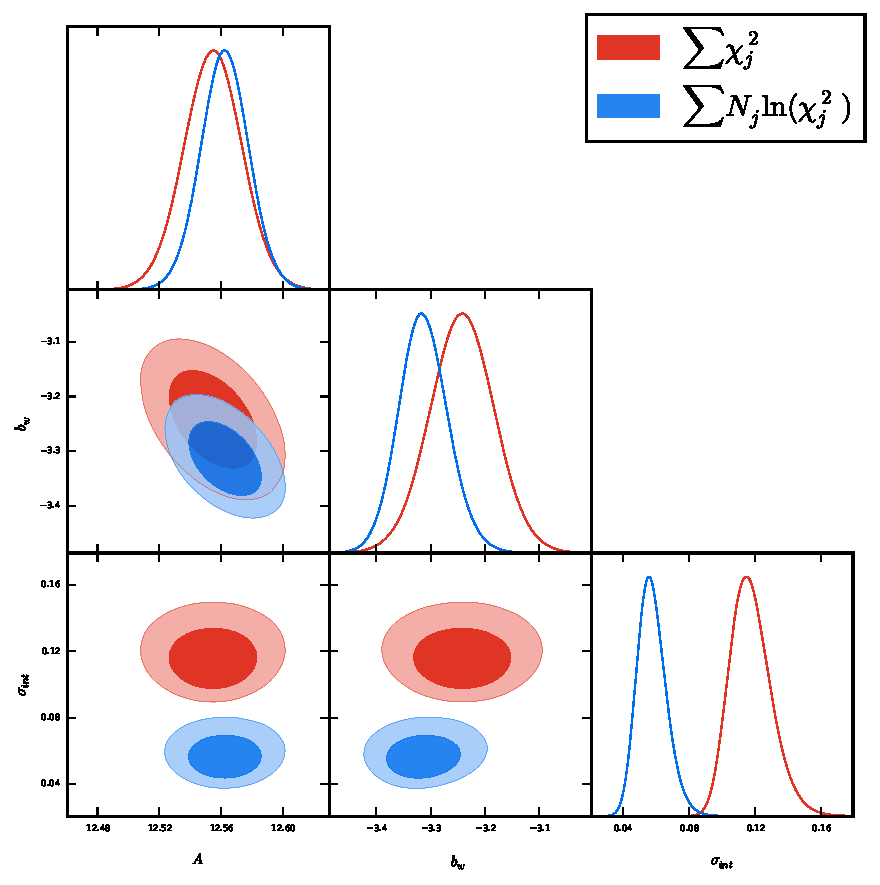
\includegraphics[scale=1]{figures/chapter-h0/triangle_figure_joint_sigma_int.pdf}
\caption{Two- and 1D posteriors for the parameters in the period-luminosity relation. Red shows a standard $\chi^2$ minimisation and blue uses HPs.  }
\label{fig:sigmaint}
\end{figure}

The LMC Cepheids are also treated as illustrative example in section 2 of \cite{Efstathiou:2013via}. This allows us to compare the approach used there, which does not use hyper-parameters, with the results found here. In our approach, the posterior mean values of $A$ and $b_W$ always lie in between the values given in \cite{Efstathiou:2013via}. They do also not depend significantly on the period cut (except that the error becomes larger for the most restrictive cut, $10<P<60$. We conclude that our treatment performs reasonably well when compared to the standard $\chi^2$ approach, and also that the hyper-parameters allow to use all the available data without significant bias. We will investigate this conclusion further as we add more data.

In Figure \ref{Fig:LMC-Cepheid-variables-fit-c} we also show the colour-coded effective HP value for all the data points in the LMC Cepheid sample, based on (\ref{Eq:effective-HP-1}) and (\ref{Eq:effective-HP-2}). Especially the lower panel, where we plot the residuals with respect to the best fit, shows clearly how outliers have a lower effective hyper parameter and thus less weight. If instead we used a standard $\chi^2$ fit to all of these points (i.e.\ without period cut) then the fit would be pulled towards a steeper slow (higher $b_W$) by the green points near the extrema of $P$ as shown by the red dotted line in the upper panel of Fig. \ref{Fig:LMC-Cepheid-variables-fit-c}. 

The LMC distance modulus derived from observations of eclipsing binaries \cite{Pietrzynski:2013gia} is 
\begin{equation}
\mu_{0,\LMC}^{\obs} = 18.49 \pm 0.05\, \magn,
\label{Eq:LMC-measured-distance-modulus}
\end{equation}
that together with $A$ from Table \ref{Table:LMC-fits} for fit c gives a Cepheid zero point
\begin{equation}\label{Eq:zero-point-LMC}
M_W = -5.93 \pm 0.07\, \magn.
\end{equation}


\subsection{The MW Cepheid variables}
\label{Subsection:MW-1}

We discuss next the set of $13$ MW Cepheid stars with parallax measurements listed in Table 2 of \cite{vanLeeuwen:2007xw} (eliminating Polaris as in \cite{Efstathiou:2013via} and correcting for Lutz-Kelker bias). We consider the MW Cepheids separately here because, as we will see, the MW data pushes the inferred value of $H_0$ to higher values, and it is thus important to check whether there is a reason to discard this data set or not.

The period-luminosity relation for those Cepheid stars is given by
\begin{equation}\label{Eq:P-L-MW}
M^P_W = M_W + b_W (\log P - 1)
\end{equation}
where $Z_W=0$ in Eq. \eqref{Eq:P-L-equation}, $M^P_W = m^P_W - \mu_{\pi}$ and $\mu_\pi$ is the distance modulus derived from parallaxes. Here we define 
\begin{equation}\label{Eq:chi2-MW}
\chi^{2,\MW}_{i} = \frac{(M_{W,i} - M^P_{W})^2}{\sigma_i^2 + \sigma^{2,\MW}_{\intt}},
\end{equation}
where $\sigma_i$ is the observational error on $M_{W,i}$ and $\sigma_{\intt}^{\MW}$ is once more the internal dispersion (that we again include as a free, marginalised parameter as in the previous section on the LMC Cepheids). Maximizing  
\begin{equation}
\label{Eq:likelihood-HP-MW}
\ln P^{\MW}(M_W,b_W,\lbrace D_i \rbrace) = \sum_{i} \ln \tilde{\chi}_i^{2}(\chi^{2,\MW}_{i}) + \ln \tilde{N}^{\MW}_{i},
\end{equation}
where 
\begin{equation}
\label{Eq:normalization-MW}
\tilde{N}^{\MW}_i = \frac{1}{\sqrt{\sigma_i^2 +\sigma^{2,\MW}_{\intt}}},
\end{equation}
we find the best-fitting parameters of the period-luminosity relation \eqref{Eq:P-L-MW}. They are 
\begin{equation}\label{Eq:MW-bestfit}
M_W = -5.88 \pm 0.07\,\magn  , \qquad b_W = -3.30 \pm 0.26  , \qquad \sigma_{\intt}^{\MW} = 0.02 ,
\end{equation}
in good agreement with fits in Table \ref{Table:LMC-fits} and with \cite{Efstathiou:2013via}. 
Figure \ref{Fig:MW-Cepheid-variables} shows period-luminosity relation for the MW Cepheid variables and best fit in Eq. \eqref{Eq:MW-bestfit}.

\begin{figure}[tbp]
\centering % \begin{center}/\end{center} takes some additional vertical space
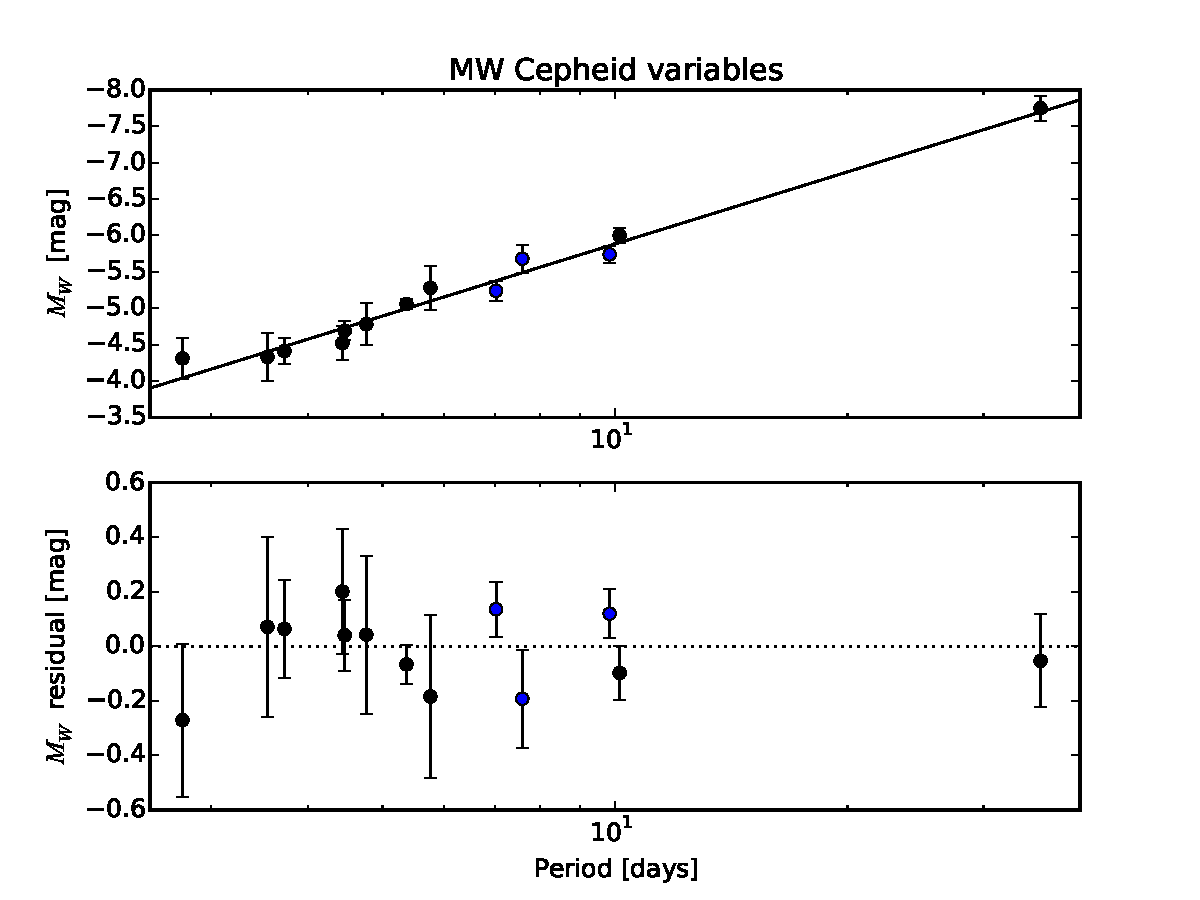
\includegraphics[scale=0.75]{figures/chapter-h0/effective_HP_cepheids_MW.pdf} 
\caption{Period-luminosity relation for the MW Cepheid variables. Upper panel shows the best fit. Error bars have been rescaled with corresponding effective HPs which are colour-coded as in Figure \ref{Fig:LMC-Cepheid-variables-fit-c}. Lower panel shows magnitude residuals; Error bars are not rescaled and colours correspond to those in upper panel.}
\label{Fig:MW-Cepheid-variables}
\end{figure}

The consistency in both the Cepheid zero point $M_W$ (Eq. \eqref{Eq:zero-point-LMC}) and the slope $b_W$ between the MW and the LMC Cepheid data, as well as the lack of marked outliers visible in Fig.\ \ref{Fig:MW-Cepheid-variables} provides no argument for excluding the MW data, at least based on the Cepheid stars. For this reason we will include the MW data in our `standard analysis' discussed in Section \ref{Subsection:combining-anchors}. We also note that the MW Cepheid data have no preference for a non-zero $\sigma^{\MW}_{\intt}$, although including it does not change the fit significantly.

\subsection{Cepheid variables in the megamaser system $\NGC$}
\label{Subsection:NGC4258}

In this subsection we use the set of $\NGC$ Cepheid variables included in the sample of \cite{Riess:2011yx} to fit the period-luminosity relation \eqref{Eq:P-L-LMC} setting now $A = \mu_{0, \NGC} + M_W$ and neglecting metallicity dependence. We find
\begin{figure}[tbp]
\centering % \begin{center}/\end{center} takes some additional vertical space
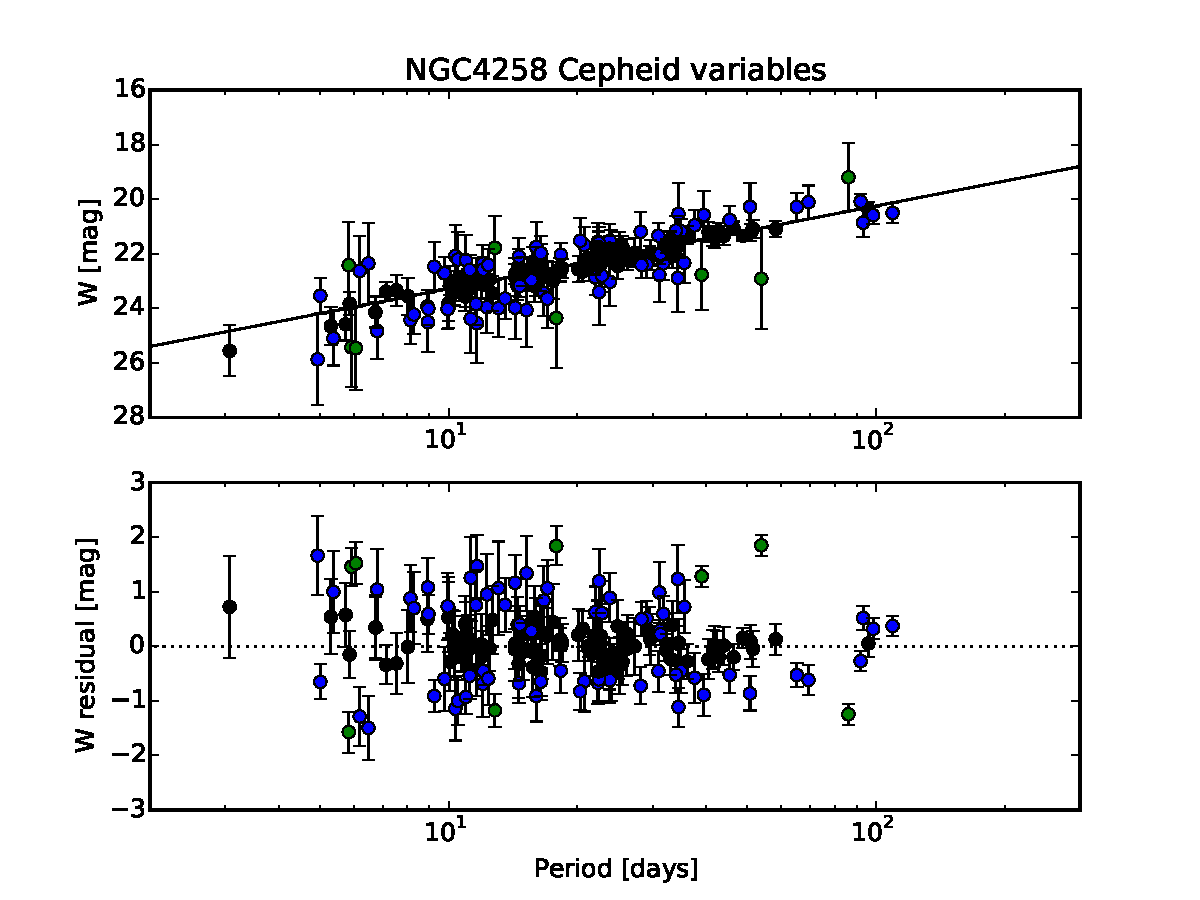
\includegraphics[scale=0.75]{figures/chapter-h0/effective_HP_cepheids_NGC4258.pdf} 
\caption{Period-luminosity relation for the $\NGC$ Cepheid variables. Upper panel shows the best fit; Error bars have been rescaled with corresponding effective HPs which are colour-coded as in Figure \ref{Fig:LMC-Cepheid-variables-fit-c}. Lower panel shows magnitude residuals; Error bars are not rescaled and colours correspond to those in upper panel.}
\label{Fig:NGC4258-Cepheid-variables}
\end{figure}

\begin{equation}\label{Eq:NGC4258-bestfit}
A = 23.281 \pm 0.078\, \magn  , \qquad b_W = -3.02 \pm 0.17  , \qquad \sigma_{\intt}^{\NGC} = 0.12 .
\end{equation}
Fig. \ref{Fig:NGC4258-Cepheid-variables} shows period-luminosity relation and residuals for the $\NGC$ Cepheid variables. Note that the slope $b_W$ for the fit \eqref{Eq:NGC4258-bestfit} is about $1.7\sigma$ away from the fit c in Table \ref{Table:LMC-fits} and the internal scatter $\sigma_{\intt}^{\NGC}=2\sigma_{\intt}^{\LMC}$. The $\NGC$ distance modulus derived from the geometric maser distance estimate to the active galaxy $\NGC$ \cite{Humphreys:2013eja} is 
\begin{equation}
\mu_{0,\NGC}^{\obs} = 29.40 \pm 0.07\, \magn,
\label{Eq:NGC4258-measured-distance-modulus-2013}
\end{equation}
which leads to a Cepheid zero point $M_W=-6.12 \pm 0.15\, \magn$, a value about $1.6\sigma$ away from that in Eq. \eqref{Eq:MW-bestfit}.\footnote{The standardised candle method for type IIP SNe \cite{Polshaw:2015ika} provides an alternative determination of the $\NGC$ distance modulus:
$\mu_{0,\NGC} = 29.25 \pm 0.26\, \magn$. Although compatible with \eqref{Eq:NGC4258-measured-distance-modulus-2013},  it is much less precise and therefore we do not include it in our analysis. }
In the next subsection we explore the possibility of whether or not a metallicity dependence in the period-luminosity relation may improve the agreement in both the Cepheid zero point $M_W$ and the slope $b_W$. 

\subsection{Metallicity dependence in the period-luminosity relation}\label{Subsection:Zw-dependence}

Although the Leavitt law is expected to depend at some level on the Cepheids metal abundance \cite{Freedman:2010xv}, thus far we have neglected this effect. Here we will study how an additional degree of freedom in the period-luminosity relation (i.e., $Z_W \neq 0$) impacts the fits we have presented. As in \cite{Efstathiou:2013via} we consider a mean metallicity $\Delta \log[O/H]=8.5$ for the LMC and $\Delta \log[O/H]=8.9$ for the MW. For all other galaxies we use the metallicity reported in Table 2 of \cite{Riess:2011yx}; Cepheid variables in those galaxies have a mean metallicity close to that of the Cepheid variables in the MW, $\Delta \log[O/H] \approx 8.9$.

Table \ref{Table:Zw-dependence-of-PL-relation} shows the fit for the period-luminosity relation \eqref{Eq:P-L-equation}  (setting $A=\mu_{0,i} + M_W$) for all the galaxies containing Cepheid variables. We notice that the effect of metallicity on both the slope $b_W$ and the Cepheid zero point $M_W$ (through its dependence on $A$) is never greater than $4.3\%$ (n3021) and $8.1\%$ (NGC4028), respectively. The metallicity parameter $Z_W$ is compatible with zero in all galaxies, its main effect being a small shift and a potentially large increase in the standard deviation of the Cepheid zero point due to a degeneracy between these two parameters (see Fig. \ref{Fig:Main-analysis-fitM1a}). 

Another important worthwhile point to note from results in Table \ref{Table:Zw-dependence-of-PL-relation} is the fact that about half of the host galaxies in the sample of \cite{Riess:2011yx} have a less steep slope $b_W$ than that of the LMC Cepheid variables, the shift being $\gtrsim 2\sigma$ for n4536, n4639, n1309, n4038, and n5584. This difference in the slope is however not improved by leaving more freedom in the metallicity dependence.

Cepheid zero point $M_W$ derived from MW Cepheids is insensitive to including metallicity dependence in the period-luminosity relation. For both LMC and $\NGC$ Cepheid variables, a small dependence on metallicity (strong prior) brings the Cepheid zero point in slightly better agreement with that derived from MW Cepheids. In particular, for the $\NGC$ distance modulus in Eq. \eqref{Eq:NGC4258-measured-distance-modulus-2013} and using a strong prior on $Z_W$, we obtain $M_W=-6.11 \pm 0.26$.

Because of the $M_W - Z_W$ degeneracy, and since the additional freedom in the metallicity dependence does not bring the different Cepheid data sets into better agreement,
we will use the `strong' prior on the metallicity, $Z_W = 0 \pm 0.02$, as our default choice.

\begin{table}[tbp]
\centering
\begin{tabular}{@{}ccccc}
\hline
\multicolumn{5}{c}{Sample of Cepheid variables} \\
\hline
galaxy & $A$ & $b_W$ & $Z_W$ & $\sigma_{\intt}$ \\
\hline
 LMC & $12.699\,(2.139)$ & $-3.31\,(0.05)$ & $-0.016\,(0.252)\,[W]$ & $0.06$ \\

LMC & $12.562\,(0.170)$ & $-3.31\,(0.05)$ & $0.000\,(0.020)\,[S]$ & $0.06$ \\
  
 MW & $-5.88\,(2.23)$ & $-3.30\,(0.26)$ & $0.000\,(0.250)\,[W]$ & $0.02$ \\

 MW & $-5.88\,(0.19)$ & $-3.30\,(0.26)$ & $0.000\,(0.020)\,[S]$ & $0.02$ \\
 
 $\NGC$ & $25.175\,(1.957)$ & $-3.00\,(0.17)$ & $-0.214\,(0.221)\,[W]$& $0.12$ \\

 $\NGC$ & $23.293\,(0.193)$ & $-3.02\,(0.17)$ & $-0.001\,(0.020)\,[S]$& $0.12$ \\
 
 n4536 & $24.620\,(1.866)$ & $-2.85\,(0.17)$ & $ 0.021\,(0.214)\,[W]$ & $0.07$ \\

 n4536 & $24.803\,(0.207)$ & $-2.84\,(0.17)$ & $ 0.000\,(0.020)\,[S]$ & $0.07$ \\
 
 n4639 & $26.572\,(1.846)$ & $-2.46\,(0.42)$ & $-0.147\,(0.210)\,[W]$ & $0.03$ \\
 
 n4639 & $25.303\,(0.302)$ & $-2.49\,(0.42)$ & $-0.001\,(0.020)\,[S]$ & $0.04$ \\
  
 n3982 & $26.591\,(1.724)$ & $-3.28\,(0.42)$ & $-0.083\,(0.200)\,[W]$ & $0.03$ \\
  
 n3982 & $25.888\,(0.283)$ & $-3.27\,(0.42)$ & $ 0.000\,(0.020)\,[S]$ & $0.03$ \\
   
 n3370 & $28.317\,(1.696)$ & $-2.99\,(0.20)$ & $-0.260\,(0.196)\,[W]$ & $0.02$ \\
 
 n3370 & $26.098\,(0.224)$ & $-3.03\,(0.20)$ & $-0.003\,(0.020)\,[S]$ & $0.02$ \\
  
 n3021 & $28.226\,(1.983)$ & $-2.86\,(0.51)$ & $-0.239\,(0.231)\,[W]$ & $0.03$ \\

 n3021 & $26.211\,(0.325)$ & $-2.99\,(0.50)$ & $-0.002\,(0.020)\,[S]$ & $0.03$ \\
  
 n1309 & $26.788\,(2.032)$ & $-2.09\,(0.42)$ & $-0.105\,(0.225)\,[W]$ & $0.03$ \\

 n1309 & $25.857\,(0.354)$ & $-2.08\,(0.42)$ & $-0.000\,(0.020)\,[S]$ & $0.03$ \\
   
 n4038 & $24.200\,(2.171)$ & $-2.47\,(0.27)$ & $0.092\,(0.243)\,[W]$ & $0.03$ \\

 n4038 & $25.011\,(0.291)$ & $-2.45\,(0.27)$ & $0.000\,(0.020)\,[S]$ & $0.03$ \\
    
 n5584 & $25.428\,(1.782)$ & $-2.83\,(0.24)$ & $0.013\,(0.204)\,[W]$ & $0.03$ \\   

 n5584 & $25.541\,(0.240)$ & $-2.83\,(0.24)$ & $0.000\,(0.020)\,[S]$ & $0.03$ \\   
 
\hline
\end{tabular}
\caption{\label{Table:Zw-dependence-of-PL-relation} Mean values and standard deviation (in brackets) in the period-luminosity relation parameters for the sample of Cepheid variables used in this work. The period range used to fit the data is the same used in fit c of Table \ref{Table:LMC-fits} ($P<205$ days). $[W]$ stands for a Gaussian prior with mean  $\bar{Z_W}=0$ and standard deviation $\sigma_{Z_W}=0.25$. $[S]$ stands for a Gaussian prior with $\bar{Z_W}=0$ and $\sigma_{Z_W}=0.02$. The internal dispersion for each galaxy is shown in the last column.}
\end{table}

\subsection{Determining the current expansion rate of the universe with Bayesian hyper-parameters (R11 data set)}
\label{Subsection:combining-anchors}

We have seen that the period-luminosity parameters independently derived from LMC, MW, and $\NGC$ Cepheid variables are in good agreement and therefore we do not see any reason to discard any of the data sets when determining the Hubble constant with hyper-parameters. In this section we use the sample of Cepheid variables for the $\SNe$ hosts from \cite{Riess:2011yx}, the set of LMC Cepheid variables used in Section \ref{Subsection:LMC} and the set of MW Cepheid variables used in Section \ref{Subsection:MW-1}. As for sources of calibration of the absolute distance scale, we utilize both the revised $\NGC$ geometric maser distance from \cite{Humphreys:2013eja} and the distance to LMC derived from observations of eclipsing binaries from \cite{Pietrzynski:2013gia}.

We use hyper parameters for all Cepheid fits as there are outliers in most of the data sets (except possibly the MW Cepheids, see Figure \ref{Fig:effective-HP-fitM1a}). Although trigonometric parallaxes to MW Cepheid variables are one of most direct source of geometric calibration for those stars, we have included them with HPs because there exists an ongoing discussion about their parallax uncertainties (see section 3.1.1 of \cite{Riess:2016jrr}).

As we will see we find that the $\SNe$ data now shows inconsistencies (see Figure \ref{Fig:HP-SNIa-main-analysis} and Table \ref{Table:SNIa-HP-fit-M1a} below), so we include it also with hyper parameters. We have however included a few cases where $\SNe$ magnitudes are included without HPs; In these cases $\SNe$ measured magnitudes are assumed being drawn from a Gaussian distribution. 

We include the available distance modulus to both $\NGC$ and LMC with hyper-parameters (especially when combining these two anchor distances in the same fit), but run a few cases including them without HPs. Note that the inclusion of these distance calibrators in our approach can be viewed as the introduction of priors on $\mu_{0,\NGC}$ and $\mu_{0,\LMC}$.  For anchor distances and SNe Ia magnitudes we then assume a Gaussian HP likelihood as in Eq. \eqref{Eq:hyper-likelihood}.

Hence in order to find the best-fitting parameters $\vec{w}$ we maximize 
\begin{equation}
\ln P(\vec{w},\lbrace D_i \rbrace) = \ln P^{\Cepheid} + \ln P^{\SNe} + \ln P^{\Anchors}. 
\end{equation}
For Cepheid variables we have, as in Subsections \ref{Subsection:LMC}-\ref{Subsection:Zw-dependence}, 
\begin{subequations}
\begin{equation}
\ln P^{\Cepheid} = \sum_{ij} \ln \tilde{\chi}^{2}(\chi^{2,\Cepheid}_{ij}) + \ln \tilde{N}^{\Cepheid}_{ij},
\end{equation}
where
\begin{equation}
\tilde{N}^{\Cepheid}_{ij} = \frac{1}{\sqrt{\sigma_{e,ij}^2 + \sigma_{\intt,i}^2}},
\end{equation}
\begin{equation}
\chi^{2,\Cepheid}_{ij} = \frac{(m_{W,ij} - m^P_{W,i,j})^2}{\sigma_{e,ij}^2 + \sigma_{\intt,i}^2},
\end{equation}
and the Cepheid magnitude is modelled as in Eq. \eqref{Eq:P-L-equation} for the passband $W$ and utilizing the ``Wesenheit reddening-free'' magnitudes 
\begin{equation}
m_{W,ij} = m_{H,ij} - R\, (m_{V,ij} - m_{I,ij})
\end{equation}
\end{subequations}
and $\sigma_{\intt,i}$, as in Subsections \ref{Subsection:LMC}-\ref{Subsection:Zw-dependence}, is the internal scatter for the $i\mathrm{th}$ galaxy (i.e., $i\mathrm{th}=\LMC,\, \MW,\,\NGC,\dots$), $j$ being the index of the Cepheid belonging to the $i\mathrm{th}$ galaxy. In this section we set $R=0.410$, but when analysing the R16 data set we study the impact of different values of $R$ in our analysis. 

For $\SNe$ magnitudes we use the likelihood
\begin{multline}
\ln P^{\SNe}  =  \sum_{i} \ln \tilde{\chi}^{2}(\chi^{2,\SNe}_{i}) + \ln \tilde{N}^{\SNe}_{i} - \frac{(a^{\rm R11}_V - a_V)^2}{2 \sigma_{a_V}^2} \\
- \frac{\ln (2\pi\sigma_{a_V}^2)}{2} - \frac{(a_{\rm cal})^2}{2 \sigma_{a_{\rm cal}}^2} - \frac{\ln (2\pi\sigma_{a_{\rm cal}}^2)}{2}  
\label{eq:ialike}
\end{multline}
where 
\begin{equation}
\tilde{N}^{\SNe}_{i} = \frac{1}{\sqrt{\sigma_{i}^2}},
\end{equation}
\begin{equation}
\chi^{2,\SNe}_{i} = \frac{(m^0_{X,i} - m^{\theo}_{X,i})^2}{\sigma_{i}^2},
\end{equation}
\begin{equation}
m^{\theo}_{X,i} = \mu_{0,i} + 5 \log H_0 - 25 - 5 a_X \, 
\end{equation}
is the $\SNe$ apparent magnitude \eqref{Eq:apparent-magnitude-H0}, and both $m^0_{X,i}$ and $\sigma_i$ are taken from the table 3 in \cite{Riess:2011yx}. Here $a_X$ is the intercept of the $\SNe$ magnitude-redshift relation, and \cite{Riess:2011yx} gives its value as $a_V = 0.697\pm0.00201$ (using wavelength $V$). We call the mean value 
in the above expression for the likelihood $a^{\rm R11}_V = 0.697$ and the uncertainty $\sigma_{a_V} = 0.00201$, and assume that $a_V$ itself has a Gaussian pdf given by these quantities. If we were dealing with Gaussian likelihood for $m^0_{V,i}$ then we could marginalize analytically over $a_V$, which would then contribute a fully correlated error to the covariance matrix for the $m^0_{V,i}$. But as we are using HPs, we instead add $a_V$ as an explicit (nuisance) parameter in Eq.\ (\ref{eq:ialike}), together with its associated Gaussian likelihood, and sample from it numerically. Similarly, we take into account the calibration error, $\sigma_{a_{\rm cal}}$, between the ground based and the WFC3 photometry by introducing a nuisance parameter $a_{\rm cal}$. We assume it has a Gaussian pdf with zero mean and $\sigma_{a_{\rm cal}}=0.04$.

Finally, motivated by the inconsistencies of distance anchors found by G. Efstathiou in  \cite{Efstathiou:2013via}, we include the available distance modulus as
\begin{equation}
\ln P^{\Anchors} = \sum_{i} \ln \tilde{\chi}^{2}\left( \chi^{2,\Anchors}_{i} \right) + \ln \tilde{N}^{\Anchors}_{i} 
\end{equation}
where
\begin{equation}
\tilde{N}^{\Anchors}_{i} = \frac{1}{\sqrt{\sigma_{i}^2}},
\end{equation}
\begin{equation}
\chi^{2,\Anchors}_i = \frac{(\mu_{0,i} - \mu^{\obs}_{0,i})^2}{\sigma^2_i},
\end{equation}
where $i=\LMC,\,\NGC$ and $\mu^{\obs}_{0,\LMC}$ and $\mu^{\obs}_{\rm 0,\NGC}$ are given by Eqs. \eqref{Eq:LMC-measured-distance-modulus} and \eqref{Eq:NGC4258-measured-distance-modulus-2013} respectively.

At this point we have assembled all ingredients necessary to determine the Hubble parameter, using HPs rather than a rejection algorithm. We have performed several variants (see Table \ref{Table:details-fits}) of the analysis that are shown in Table \ref{Table:Constraints-main-analysis}.

%\begin{table}[tbp]
%\centering
%\resizebox{14.cm}{!}{
%\begin{tabular}{lcccccccccccccr}
%\hline 
%\rule[-1ex]{0pt}{2.5ex} fit & $\alpha^{\Cepheid}$ & $\alpha^{\SNe}$ & $\alpha^{\Anchors}$ & $P$ & $R$ & $\sigma_{Z_W}$ & $\sigma_{\intt,i}$ & $\sigma_{\intt}^{\LMC}$ & $\sigma_{\intt}^{\MW}$ & CS & $\mu_{0,\NGC}^{\obs}$ & $\mu_{0,\LMC}^{\obs}$ & $\mu_{0,\MAnd}^{\obs}$ & $\MW$ \\ 
%\hline 
%\rule[-1ex]{0pt}{2.5ex} $1$ & Y & Y & Y & $205$ & $0.410$ & - & V & V & - & R11 & \cite{Humphreys:2013eja} & - & - & - \\ 
%\rule[-1ex]{0pt}{2.5ex} $2$ & Y & Y & Y & $60$ & $0.410$ & - & V & V & - & R11 & \cite{Humphreys:2013eja} & - & - & - \\ 
%\rule[-1ex]{0pt}{2.5ex} $3$ & Y & Y & Y & $205$ & $0.410$ & $0.02$ & V & V & - & R11 & \cite{Humphreys:2013eja} & - & - & - \\ 
%\rule[-1ex]{0pt}{2.5ex} $4$ & Y & Y & N & $205$ & $0.410$ & $0.02$ & V & V & - & R11 & \cite{Humphreys:2013eja} & - & - & - \\ 
%\rule[-1ex]{0pt}{2.5ex} $5$ & Y & Y & Y & $60$ & $0.410$ & $0.02$ & V & V & - & R11 & \cite{Humphreys:2013eja} & - & - & - \\ 
%\rule[-1ex]{0pt}{2.5ex} $6$ & Y & Y & N & $60$ & $0.410$ & $0.02$ & V & V & - & R11 & \cite{Humphreys:2013eja} & - & - & - \\ 
%\rule[-1ex]{0pt}{2.5ex} $7$ & Y & Y & Y & $205$ & $0.410$ & - & V & V & - & R11 & - & \cite{Pietrzynski:2013gia} & - & - \\ 
%\rule[-1ex]{0pt}{2.5ex} $8$ & Y & Y & Y & $60$ & $0.410$ & - & V & V & - & R11 & - & \cite{Pietrzynski:2013gia} & - & - \\ 
%\rule[-1ex]{0pt}{2.5ex} $9$ & Y & Y & Y & $205$ & $0.410$ & $0.02$ & V & V & - & R11 & - & \cite{Pietrzynski:2013gia} & - & - \\ 
%\rule[-1ex]{0pt}{2.5ex} $10$ & Y & Y & N & $205$ & $0.410$ & $0.02$ & V & V & - & R11 & - & \cite{Pietrzynski:2013gia} & - & - \\ 
%\rule[-1ex]{0pt}{2.5ex} $11$ & Y & Y & Y & $60$ & $0.410$ & $0.02$ & V & V & - & R11 & - & \cite{Pietrzynski:2013gia} & - & - \\ 
%\rule[-1ex]{0pt}{2.5ex} $12$ & Y & Y & N & $60$ & $0.410$ & $0.02$ & V & V & - & R11 & - & \cite{Pietrzynski:2013gia} & - & - \\ 
%\rule[-1ex]{0pt}{2.5ex} $13$ & Y & Y & - & $205$ & $0.410$ & - & V & V & V & R11 & - & - & - & \cite{vanLeeuwen:2007xw} \\ 
%\rule[-1ex]{0pt}{2.5ex} $14$ & Y & Y & - & $60$ & $0.410$ & - & V & V & V & R11 & - & - & - & \cite{vanLeeuwen:2007xw} \\
%\rule[-1ex]{0pt}{2.5ex} $15$ & Y & Y & - & $205$ & $0.410$ & $0.02$ & V & V & V & R11 & - & - & - & \cite{vanLeeuwen:2007xw} \\
%\rule[-1ex]{0pt}{2.5ex} $16$ & Y & Y & - & $60$ & $0.410$ & $0.02$ & V & V & V & R11 & - & - & - & \cite{vanLeeuwen:2007xw} \\
%\rule[-1ex]{0pt}{2.5ex} $17$ & Y & Y & Y & $205$ & $0.410$ & - & V & V & - & R11 & \cite{Humphreys:2013eja} & \cite{Pietrzynski:2013gia} & - & - \\
%\rule[-1ex]{0pt}{2.5ex} $18$ & Y & Y & Y & $60$ & $0.410$ & - & V & V & - & R11 & \cite{Humphreys:2013eja} & \cite{Pietrzynski:2013gia} & - & - \\
%\rule[-1ex]{0pt}{2.5ex} $19$ & Y & Y & Y & $205$ & $0.410$ & $0.02$ & V & V & - & R11 & \cite{Humphreys:2013eja} & \cite{Pietrzynski:2013gia} & - & - \\
%\rule[-1ex]{0pt}{2.5ex} $20$ & Y & Y & Y & $60$ & $0.410$ & $0.02$ & V & V & - & R11 & \cite{Humphreys:2013eja} & \cite{Pietrzynski:2013gia} & - & - \\
%\rule[-1ex]{0pt}{2.5ex} $21$ & Y & Y & Y & $205$ & $0.410$ & - & V & V & V & R11 & \cite{Humphreys:2013eja} & - & - & \cite{vanLeeuwen:2007xw} \\ 
%\rule[-1ex]{0pt}{2.5ex} $22$ & Y & Y & Y & $60$ & $0.410$ & - & V & V & V & R11 & \cite{Humphreys:2013eja} & - & - & \cite{vanLeeuwen:2007xw} \\
%\rule[-1ex]{0pt}{2.5ex} $23$ & Y & Y & Y & $205$ & $0.410$ & $0.02$ & V & V & V & R11 & \cite{Humphreys:2013eja} & - & - & \cite{vanLeeuwen:2007xw} \\
%\rule[-1ex]{0pt}{2.5ex} $24$ & Y & Y & Y & $60$ & $0.410$ & $0.02$ & V & V & V & R11 & \cite{Humphreys:2013eja} & - & - & \cite{vanLeeuwen:2007xw} \\
%\rule[-1ex]{0pt}{2.5ex} $25$ & Y & Y & Y & $205$ & $0.410$ & - & V & V & V & R11 & - & \cite{Pietrzynski:2013gia} & - & \cite{vanLeeuwen:2007xw} \\ 
%\rule[-1ex]{0pt}{2.5ex} $26$ & Y & Y & Y & $60$ & $0.410$ & - & V & V & V & R11 & - & \cite{Pietrzynski:2013gia} & - & \cite{vanLeeuwen:2007xw} \\
%\rule[-1ex]{0pt}{2.5ex} $27$ & Y & Y & Y & $205$ & $0.410$ & $0.02$ & V & V & V & R11 & - & \cite{Pietrzynski:2013gia} & - & \cite{vanLeeuwen:2007xw} \\
%\rule[-1ex]{0pt}{2.5ex} $28$ & Y & Y & Y & $60$ & $0.410$ & $0.02$ & V & V & V & R11 & - & \cite{Pietrzynski:2013gia} & - & \cite{vanLeeuwen:2007xw} \\
%
%\rule[-1ex]{0pt}{2.5ex} $29$ & Y & Y & Y & $205$ & $0.410$ & $0.02$ & V & V & V & R11 & \cite{Humphreys:2013eja} & \cite{Pietrzynski:2013gia} & - & \cite{vanLeeuwen:2007xw} \\ 
%\rule[-1ex]{0pt}{2.5ex} $30$ & Y & Y & Y & $205$ & $0.410$ & $0.02$ & V & V & V & R11 & \cite{Humphreys:2013eja} & \cite{Pietrzynski:2013gia} & - & \cite{vanLeeuwen:2007xw} \\
%\rule[-1ex]{0pt}{2.5ex} $31$ & Y & N & Y & $205$ & $0.410$ & $0.02$ & V & V & V & R11 & \cite{Humphreys:2013eja} & \cite{Pietrzynski:2013gia} & - & \cite{vanLeeuwen:2007xw} \\
%\rule[-1ex]{0pt}{2.5ex} $32$ & Y & Y & N & $205$ & $0.410$ & $0.02$ & V & V & V & R11 & \cite{Humphreys:2013eja} & \cite{Pietrzynski:2013gia} & - & \cite{vanLeeuwen:2007xw} \\
%\rule[-1ex]{0pt}{2.5ex} $33$ & Y & N & N & $205$ & $0.410$ & $0.02$ & V & V & V & R11 & \cite{Humphreys:2013eja} & \cite{Pietrzynski:2013gia} & - & \cite{vanLeeuwen:2007xw} \\
%\rule[-1ex]{0pt}{2.5ex} $34$ & Y & Y & Y & $60$ & $0.410$ & $0.02$ & V & V & V & R11 & \cite{Humphreys:2013eja} & \cite{Pietrzynski:2013gia} & - & \cite{vanLeeuwen:2007xw} \\
%\rule[-1ex]{0pt}{2.5ex} $35$ & Y & N & N & $60$ & $0.410$ & $0.02$ & $0.30$ & $0.113$ & $0.10$ & R11 & \cite{Humphreys:2013eja} & \cite{Pietrzynski:2013gia} & - & \cite{vanLeeuwen:2007xw} \\
%\rule[-1ex]{0pt}{2.5ex} $36$ & Y & Y & Y & $205$ & $0.410$ & $0.25$ & V & V & V & R11 & \cite{Humphreys:2013eja} & \cite{Pietrzynski:2013gia} & - & \cite{vanLeeuwen:2007xw} \\
%\rule[-1ex]{0pt}{2.5ex} $37$ & Y & Y & Y & $60$ & $0.410$ & $0.25$ & V & V & V & R11 & \cite{Humphreys:2013eja} & \cite{Pietrzynski:2013gia} & - & \cite{vanLeeuwen:2007xw} \\
%\rule[-1ex]{0pt}{2.5ex} $38$ & Y & Y & Y & $205$ & $0.410$ & - & V & V & V & R11 & \cite{Humphreys:2013eja} & \cite{Pietrzynski:2013gia} & - & \cite{vanLeeuwen:2007xw} \\
%\rule[-1ex]{0pt}{2.5ex} $39$ & Y & Y & Y & $60$ & $0.410$ & - & V & V & V & R11 & \cite{Humphreys:2013eja} & \cite{Pietrzynski:2013gia} & - & \cite{vanLeeuwen:2007xw} \\ 
%
%%R16 STARTS HERE
%\rule[-1ex]{0pt}{2.5ex} $12$ & Y & Y & Y & $205$ & $0. $ & - & - & - & - & R16 & \cite{Riess:2016jrr} & \cite{Pietrzynski:2013gia} & \cite{Riess:2016jrr} & \cite{Riess:2016jrr} \\ 
%\rule[-1ex]{0pt}{2.5ex} $13$ & Y & Y & Y & $60$ & $0. $ & - & - & - & - & R16 & \cite{Riess:2016jrr} & \cite{Pietrzynski:2013gia} & \cite{Riess:2016jrr} & \cite{Riess:2016jrr} \\
%\rule[-1ex]{0pt}{2.5ex} $14$ & Y & Y & Y & $205$ & $0. $ & $0.25$ & - & - & - & R16 & \cite{Riess:2016jrr} & \cite{Pietrzynski:2013gia} & \cite{Riess:2016jrr} & \cite{Riess:2016jrr} \\
%\rule[-1ex]{0pt}{2.5ex} $15$ & Y & Y & Y & $60$ & $0. $ & $0.25$ & - & - & - & R16 & \cite{Riess:2016jrr} & \cite{Pietrzynski:2013gia} & \cite{Riess:2016jrr} & \cite{Riess:2016jrr} \\
%\rule[-1ex]{0pt}{2.5ex} $16$ & Y & Y & Y & $205$ & $0. $ & $0.02$ & - & - & - & R16 & \cite{Riess:2016jrr} & \cite{Pietrzynski:2013gia} & \cite{Riess:2016jrr} & \cite{Riess:2016jrr} \\
%\rule[-1ex]{0pt}{2.5ex} $17$ & Y & Y & Y & $60$ & $0. $ & $0.02$ & - & - & - & R16 & \cite{Riess:2016jrr} & \cite{Pietrzynski:2013gia} & \cite{Riess:2016jrr} & \cite{Riess:2016jrr} \\
%\rule[-1ex]{0pt}{2.5ex} $18$ & Y & Y & N & $205$ & $0. $ & - & - & - & - & R16 & \cite{Riess:2016jrr} & \cite{Pietrzynski:2013gia} & \cite{Riess:2016jrr} & \cite{Riess:2016jrr} \\
%\rule[-1ex]{0pt}{2.5ex} $19$ & Y & N & Y & $205$ & $0. $ & - & - & - & - & R16 & \cite{Riess:2016jrr} & \cite{Pietrzynski:2013gia} & \cite{Riess:2016jrr} & \cite{Riess:2016jrr} \\  
%\rule[-1ex]{0pt}{2.5ex} $20$ & Y & N & N & $205$ & $0. $ & - & - & - & - & R16 & \cite{Riess:2016jrr} & \cite{Pietrzynski:2013gia} & \cite{Riess:2016jrr} & \cite{Riess:2016jrr} \\ 
%\hline
%\end{tabular}}
%\caption{$\alpha^\Cepheid$: Cepheid stars included with HPs. $\alpha^\SNe$: $\SNe$ magnitudes included with HPs. $\alpha^\Anchors$: distance moduli of anchors included with HPs; '-' stands for no distance moduli included in the fit. In columns $2-4$ 'Y' stands for 'Yes' and 'N' stands for 'No'. $P$: upper period cutoff. $R$: reddening law. $\sigma_{Z_W}$: standard deviation of the Gaussian prior on the metallicity parameter $Z_W$; '-' stands for a flat, wide prior. $\sigma_{\intt,i}$: internal dispersion for $\SNe$ hosts; 'V' stands for varying and marginalised; when the numerical value is given it means fixed internal dispersion was used; '-' stands for no internal dispersion included in the fit. $\sigma_{\intt}^{\LMC}$: $\LMC$ internal dispersion. $\sigma_{\intt}^{\MW}$: $\MW$ internal dispersion. CS: Cepheid sample. Columns $\mu_{0,\NGC}^{\obs}$, $\mu_{0,\LMC}^{\obs}$, and $\mu_{0,\MAnd}^{\obs}$ refer to references from this quantities were taken; '-' means that the data was not used in the fit. $\MW$ refers to the reference for $\MW$ Cepheid stars; '-' means that the data was not used in the fit. \label{Table:details-fits}}
%\end{table}

\begin{center}
\tiny
\setlength\LTleft{-30pt}
\setlength\LTright{-30pt}
\begin{longtable}{@{\extracolsep{\fill}}ccccccccccccccc@{}}
\caption{$\alpha^\Cepheid$: Cepheid stars included with HPs. $\alpha^\SNe$: $\SNe$ magnitudes included with HPs. $\alpha^\Anchors$: distance moduli of anchors included with HPs; '-' stands for no distance moduli included in the fit. In columns $2-4$ 'Y' stands for 'Yes' and 'N' stands for 'No'. $P$: upper period cutoff. $R$: reddening law. $\sigma_{Z_W}$: standard deviation of the Gaussian prior on the metallicity parameter $Z_W$; '-' stands for a flat, wide prior. $\sigma_{\intt,i}$: internal dispersion for $\SNe$ hosts; 'V' stands for varying and marginalised; when the numerical value is given it means fixed internal dispersion was used; '-' stands for no internal dispersion included in the fit. $\sigma_{\intt}^{\LMC}$: $\LMC$ internal dispersion. $\sigma_{\intt}^{\MW}$: $\MW$ internal dispersion. CS: Cepheid sample. Columns $\mu_{0,\NGC}^{\obs}$, $\mu_{0,\LMC}^{\obs}$, and $\mu_{0,\MAnd}^{\obs}$ refer to references from this quantities were taken; '-' means that the data was not used in the fit. $\MW$ refers to the reference for $\MW$ Cepheid stars; '-' means that the data was not used in the fit. \label{Table:details-fits}}\\
%\caption[Feasible triples for a highly variable Grid]{Feasible triples for 
%highly variable Grid, MLMMH.} \label{grid_mlmmh} \\

\hline 
fit & $\alpha^{\Cepheid}$ & $\alpha^{\SNe}$ & $\alpha^{\Anchors}$ & $P$ & $R$ & $\sigma_{Z_W}$ & $\sigma_{\intt,i}$ & $\sigma_{\intt}^{\LMC}$ & $\sigma_{\intt}^{\MW}$ & CS & $\mu_{0,\NGC}^{\obs}$ & $\mu_{0,\LMC}^{\obs}$ & $\mu_{0,\MAnd}^{\obs}$ & $\MW$ \\ 
\hline

%\hline 
%\multicolumn{1}{|c|}{\textbf{Time (s)}} & \multicolumn{1}{c|}{\textbf{Triple chosen}} & \multicolumn{1}{c|}{\textbf{Other feasible triples}} \\ \hline 
\endfirsthead

\multicolumn{15}{c}%
{{\bfseries \tablename\ \thetable{} -- continued from previous page}} \\
%\hline \multicolumn{1}{|c|}{\textbf{Time (s)}} &
%\multicolumn{1}{c|}{\textbf{Triple chosen}} &
%\multicolumn{1}{c|}{\textbf{Other feasible triples}} \\ \hline 
\hline 
fit & $\alpha^{\Cepheid}$ & $\alpha^{\SNe}$ & $\alpha^{\Anchors}$ & $P$ & $R$ & $\sigma_{Z_W}$ & $\sigma_{\intt,i}$ & $\sigma_{\intt}^{\LMC}$ & $\sigma_{\intt}^{\MW}$ & CS & $\mu_{0,\NGC}^{\obs}$ & $\mu_{0,\LMC}^{\obs}$ & $\mu_{0,\MAnd}^{\obs}$ & $\MW$ \\ 
\hline
\endhead

\hline \multicolumn{15}{c}{{Continued on next page}} \\ \hline
\endfoot

\hline \hline
\endlastfoot
%NGC4258
\rule[-1ex]{0pt}{2.5ex} $1$ & Y & Y & Y & $205$ & $0.410$ & - & V & V & - & R11 & \cite{Humphreys:2013eja} & - & - & - \\ 
\rule[-1ex]{0pt}{2.5ex} $2$ & Y & Y & Y & $60$ & $0.410$ & - & V & V & - & R11 & \cite{Humphreys:2013eja} & - & - & - \\ 
\rule[-1ex]{0pt}{2.5ex} $3$ & Y & Y & Y & $205$ & $0.410$ & $0.02$ & V & V & - & R11 & \cite{Humphreys:2013eja} & - & - & - \\ 
\rule[-1ex]{0pt}{2.5ex} $4$ & Y & Y & N & $205$ & $0.410$ & $0.02$ & V & V & - & R11 & \cite{Humphreys:2013eja} & - & - & - \\ 
\rule[-1ex]{0pt}{2.5ex} $5$ & Y & Y & Y & $60$ & $0.410$ & $0.02$ & V & V & - & R11 & \cite{Humphreys:2013eja} & - & - & - \\ 
\rule[-1ex]{0pt}{2.5ex} $6$ & Y & Y & N & $60$ & $0.410$ & $0.02$ & V & V & - & R11 & \cite{Humphreys:2013eja} & - & - & - \\ 
% LMC
\rule[-1ex]{0pt}{2.5ex} $7$ & Y & Y & Y & $205$ & $0.410$ & - & V & V & - & R11 & - & \cite{Pietrzynski:2013gia} & - & - \\ 
\rule[-1ex]{0pt}{2.5ex} $8$ & Y & Y & Y & $60$ & $0.410$ & - & V & V & - & R11 & - & \cite{Pietrzynski:2013gia} & - & - \\ 
\rule[-1ex]{0pt}{2.5ex} $9$ & Y & Y & Y & $205$ & $0.410$ & $0.02$ & V & V & - & R11 & - & \cite{Pietrzynski:2013gia} & - & - \\ 
\rule[-1ex]{0pt}{2.5ex} $10$ & Y & Y & N & $205$ & $0.410$ & $0.02$ & V & V & - & R11 & - & \cite{Pietrzynski:2013gia} & - & - \\ 
\rule[-1ex]{0pt}{2.5ex} $11$ & Y & Y & Y & $60$ & $0.410$ & $0.02$ & V & V & - & R11 & - & \cite{Pietrzynski:2013gia} & - & - \\ 
\rule[-1ex]{0pt}{2.5ex} $12$ & Y & Y & N & $60$ & $0.410$ & $0.02$ & V & V & - & R11 & - & \cite{Pietrzynski:2013gia} & - & - \\
% MW 
\rule[-1ex]{0pt}{2.5ex} $13$ & Y & Y & - & $205$ & $0.410$ & - & V & V & V & R11 & - & - & - & \cite{vanLeeuwen:2007xw} \\ 
\rule[-1ex]{0pt}{2.5ex} $14$ & Y & Y & - & $60$ & $0.410$ & - & V & V & V & R11 & - & - & - & \cite{vanLeeuwen:2007xw} \\
\rule[-1ex]{0pt}{2.5ex} $15$ & Y & Y & - & $205$ & $0.410$ & $0.02$ & V & V & V & R11 & - & - & - & \cite{vanLeeuwen:2007xw} \\
\rule[-1ex]{0pt}{2.5ex} $16$ & Y & Y & - & $60$ & $0.410$ & $0.02$ & V & V & V & R11 & - & - & - & \cite{vanLeeuwen:2007xw} \\
% NGC4258 + LMC
\rule[-1ex]{0pt}{2.5ex} $17$ & Y & Y & Y & $205$ & $0.410$ & - & V & V & - & R11 & \cite{Humphreys:2013eja} & \cite{Pietrzynski:2013gia} & - & - \\
\rule[-1ex]{0pt}{2.5ex} $18$ & Y & Y & Y & $60$ & $0.410$ & - & V & V & - & R11 & \cite{Humphreys:2013eja} & \cite{Pietrzynski:2013gia} & - & - \\
\rule[-1ex]{0pt}{2.5ex} $19$ & Y & Y & Y & $205$ & $0.410$ & $0.02$ & V & V & - & R11 & \cite{Humphreys:2013eja} & \cite{Pietrzynski:2013gia} & - & - \\
\rule[-1ex]{0pt}{2.5ex} $20$ & Y & Y & Y & $60$ & $0.410$ & $0.02$ & V & V & - & R11 & \cite{Humphreys:2013eja} & \cite{Pietrzynski:2013gia} & - & - \\ 
% NGC4258 + MW
\rule[-1ex]{0pt}{2.5ex} $21$ & Y & Y & Y & $205$ & $0.410$ & - & V & V & V & R11 & \cite{Humphreys:2013eja} & - & - & \cite{vanLeeuwen:2007xw} \\ 
\rule[-1ex]{0pt}{2.5ex} $22$ & Y & Y & Y & $60$ & $0.410$ & - & V & V & V & R11 & \cite{Humphreys:2013eja} & - & - & \cite{vanLeeuwen:2007xw} \\
\rule[-1ex]{0pt}{2.5ex} $23$ & Y & Y & Y & $205$ & $0.410$ & $0.02$ & V & V & V & R11 & \cite{Humphreys:2013eja} & - & - & \cite{vanLeeuwen:2007xw} \\
\rule[-1ex]{0pt}{2.5ex} $24$ & Y & Y & Y & $60$ & $0.410$ & $0.02$ & V & V & V & R11 & \cite{Humphreys:2013eja} & - & - & \cite{vanLeeuwen:2007xw} \\
% LMC + MW
\rule[-1ex]{0pt}{2.5ex} $25$ & Y & Y & Y & $205$ & $0.410$ & - & V & V & V & R11 & - & \cite{Pietrzynski:2013gia} & - & \cite{vanLeeuwen:2007xw} \\ 
\rule[-1ex]{0pt}{2.5ex} $26$ & Y & Y & Y & $60$ & $0.410$ & - & V & V & V & R11 & - & \cite{Pietrzynski:2013gia} & - & \cite{vanLeeuwen:2007xw} \\
\rule[-1ex]{0pt}{2.5ex} $27$ & Y & Y & Y & $205$ & $0.410$ & $0.02$ & V & V & V & R11 & - & \cite{Pietrzynski:2013gia} & - & \cite{vanLeeuwen:2007xw} \\
\rule[-1ex]{0pt}{2.5ex} $28$ & Y & Y & Y & $60$ & $0.410$ & $0.02$ & V & V & V & R11 & - & \cite{Pietrzynski:2013gia} & - & \cite{vanLeeuwen:2007xw} \\
% LMC + MW + NGC4258
\rule[-1ex]{0pt}{2.5ex} $29$ & Y & Y & Y & $205$ & $0.410$ & $0.02$ & V & V & V & R11 & \cite{Humphreys:2013eja} & \cite{Pietrzynski:2013gia} & - & \cite{vanLeeuwen:2007xw} \\ 
\rule[-1ex]{0pt}{2.5ex} $30$ & Y & Y & Y & $205$ & $0.410$ & $0.02$ & V & V & V & R11 & \cite{Humphreys:2013eja} & \cite{Pietrzynski:2013gia} & - & \cite{vanLeeuwen:2007xw} \\
\rule[-1ex]{0pt}{2.5ex} $31$ & Y & N & Y & $205$ & $0.410$ & $0.02$ & V & V & V & R11 & \cite{Humphreys:2013eja} & \cite{Pietrzynski:2013gia} & - & \cite{vanLeeuwen:2007xw} \\
\rule[-1ex]{0pt}{2.5ex} $32$ & Y & Y & N & $205$ & $0.410$ & $0.02$ & V & V & V & R11 & \cite{Humphreys:2013eja} & \cite{Pietrzynski:2013gia} & - & \cite{vanLeeuwen:2007xw} \\
\rule[-1ex]{0pt}{2.5ex} $33$ & Y & N & N & $205$ & $0.410$ & $0.02$ & V & V & V & R11 & \cite{Humphreys:2013eja} & \cite{Pietrzynski:2013gia} & - & \cite{vanLeeuwen:2007xw} \\
\rule[-1ex]{0pt}{2.5ex} $34$ & Y & Y & Y & $60$ & $0.410$ & $0.02$ & V & V & V & R11 & \cite{Humphreys:2013eja} & \cite{Pietrzynski:2013gia} & - & \cite{vanLeeuwen:2007xw} \\
\rule[-1ex]{0pt}{2.5ex} $35$ & Y & N & N & $60$ & $0.410$ & $0.02$ & $0.30$ & $0.113$ & $0.10$ & R11 & \cite{Humphreys:2013eja} & \cite{Pietrzynski:2013gia} & - & \cite{vanLeeuwen:2007xw} \\
\rule[-1ex]{0pt}{2.5ex} $36$ & Y & Y & Y & $205$ & $0.410$ & $0.25$ & V & V & V & R11 & \cite{Humphreys:2013eja} & \cite{Pietrzynski:2013gia} & - & \cite{vanLeeuwen:2007xw} \\
\rule[-1ex]{0pt}{2.5ex} $37$ & Y & Y & Y & $60$ & $0.410$ & $0.25$ & V & V & V & R11 & \cite{Humphreys:2013eja} & \cite{Pietrzynski:2013gia} & - & \cite{vanLeeuwen:2007xw} \\
\rule[-1ex]{0pt}{2.5ex} $38$ & Y & Y & Y & $205$ & $0.410$ & - & V & V & V & R11 & \cite{Humphreys:2013eja} & \cite{Pietrzynski:2013gia} & - & \cite{vanLeeuwen:2007xw} \\
\rule[-1ex]{0pt}{2.5ex} $39$ & Y & Y & Y & $60$ & $0.410$ & - & V & V & V & R11 & \cite{Humphreys:2013eja} & \cite{Pietrzynski:2013gia} & - & \cite{vanLeeuwen:2007xw} \\ 

%R16 STARTS HERE
\rule[-1ex]{0pt}{2.5ex} $40$ & Y & Y & Y & $205$ & $0.31 $ & $0.25$ & - & - & - & R16 & \cite{Riess:2016jrr} & \cite{Pietrzynski:2013gia} & \cite{Riess:2016jrr} & \cite{Riess:2016jrr} \\ 
\rule[-1ex]{0pt}{2.5ex} $41$ & Y & Y & Y & $205$ & $0.31 $ & $0.02$ & - & - & - & R16 & \cite{Riess:2016jrr} & \cite{Pietrzynski:2013gia} & \cite{Riess:2016jrr} & \cite{Riess:2016jrr} \\
\rule[-1ex]{0pt}{2.5ex} $42$ & Y & Y & Y & $205$ & $0.35 $ & $0.25$ & - & - & - & R16 & \cite{Riess:2016jrr} & \cite{Pietrzynski:2013gia} & \cite{Riess:2016jrr} & \cite{Riess:2016jrr} \\
\rule[-1ex]{0pt}{2.5ex} $43$ & Y & Y & Y & $205$ & $0.39 $ & $0.25$ & - & - & - & R16 & \cite{Riess:2016jrr} & \cite{Pietrzynski:2013gia} & \cite{Riess:2016jrr} & \cite{Riess:2016jrr} \\
\rule[-1ex]{0pt}{2.5ex} $44$ & Y & Y & Y & $205$ & $0.47 $ & $0.25$ & - & - & - & R16 & \cite{Riess:2016jrr} & \cite{Pietrzynski:2013gia} & \cite{Riess:2016jrr} & \cite{Riess:2016jrr} \\
\rule[-1ex]{0pt}{2.5ex} $45$ & Y & Y & Y & $205$ & $0.35 $ & $0.02$ & - & - & - & R16 & \cite{Riess:2016jrr} & \cite{Pietrzynski:2013gia} & \cite{Riess:2016jrr} & \cite{Riess:2016jrr} \\
\rule[-1ex]{0pt}{2.5ex} $46$ & Y & Y & Y & $205$ & $0.39 $ & $0.02$ & - & - & - & R16 & \cite{Riess:2016jrr} & \cite{Pietrzynski:2013gia} & \cite{Riess:2016jrr} & \cite{Riess:2016jrr} \\
\rule[-1ex]{0pt}{2.5ex} $47$ & Y & Y & Y & $205$ & $0.47 $ & $0.02$ & - & - & - & R16 & \cite{Riess:2016jrr} & \cite{Pietrzynski:2013gia} & \cite{Riess:2016jrr} & \cite{Riess:2016jrr} \\

\rule[-1ex]{0pt}{2.5ex} $48$ & Y & Y & Y & $60$ & $0.31 $ & $0.25$ & - & - & - & R16 & \cite{Riess:2016jrr} & \cite{Pietrzynski:2013gia} & \cite{Riess:2016jrr} & \cite{Riess:2016jrr} \\ 
\rule[-1ex]{0pt}{2.5ex} $49$ & Y & Y & Y & $60$ & $0.31 $ & $0.02$ & - & - & - & R16 & \cite{Riess:2016jrr} & \cite{Pietrzynski:2013gia} & \cite{Riess:2016jrr} & \cite{Riess:2016jrr} \\
\rule[-1ex]{0pt}{2.5ex} $50$ & Y & Y & Y & $60$ & $0.35 $ & $0.25$ & - & - & - & R16 & \cite{Riess:2016jrr} & \cite{Pietrzynski:2013gia} & \cite{Riess:2016jrr} & \cite{Riess:2016jrr} \\
\rule[-1ex]{0pt}{2.5ex} $51$ & Y & Y & Y & $60$ & $0.39 $ & $0.25$ & - & - & - & R16 & \cite{Riess:2016jrr} & \cite{Pietrzynski:2013gia} & \cite{Riess:2016jrr} & \cite{Riess:2016jrr} \\
\rule[-1ex]{0pt}{2.5ex} $52$ & Y & Y & Y & $60$ & $0.47 $ & $0.25$ & - & - & - & R16 & \cite{Riess:2016jrr} & \cite{Pietrzynski:2013gia} & \cite{Riess:2016jrr} & \cite{Riess:2016jrr} \\
\rule[-1ex]{0pt}{2.5ex} $53$ & Y & Y & Y & $60$ & $0.35 $ & $0.02$ & - & - & - & R16 & \cite{Riess:2016jrr} & \cite{Pietrzynski:2013gia} & \cite{Riess:2016jrr} & \cite{Riess:2016jrr} \\
\rule[-1ex]{0pt}{2.5ex} $54$ & Y & Y & Y & $60$ & $0.39 $ & $0.02$ & - & - & - & R16 & \cite{Riess:2016jrr} & \cite{Pietrzynski:2013gia} & \cite{Riess:2016jrr} & \cite{Riess:2016jrr} \\
\rule[-1ex]{0pt}{2.5ex} $55$ & Y & Y & Y & $60$ & $0.47 $ & $0.02$ & - & - & - & R16 & \cite{Riess:2016jrr} & \cite{Pietrzynski:2013gia} & \cite{Riess:2016jrr} & \cite{Riess:2016jrr} \\

%\rule[-1ex]{0pt}{2.5ex} $17$ & Y & Y & Y & $60$ & $0. $ & $0.02$ & - & - & - & R16 & \cite{Riess:2016jrr} & \cite{Pietrzynski:2013gia} & \cite{Riess:2016jrr} & \cite{Riess:2016jrr} \\
%\rule[-1ex]{0pt}{2.5ex} $18$ & Y & Y & N & $205$ & $0. $ & - & - & - & - & R16 & \cite{Riess:2016jrr} & \cite{Pietrzynski:2013gia} & \cite{Riess:2016jrr} & \cite{Riess:2016jrr} \\
%\rule[-1ex]{0pt}{2.5ex} $19$ & Y & N & Y & $205$ & $0. $ & - & - & - & - & R16 & \cite{Riess:2016jrr} & \cite{Pietrzynski:2013gia} & \cite{Riess:2016jrr} & \cite{Riess:2016jrr} \\  
%\rule[-1ex]{0pt}{2.5ex} $20$ & Y & N & N & $205$ & $0. $ & - & - & - & - & R16 & \cite{Riess:2016jrr} & \cite{Pietrzynski:2013gia} & \cite{Riess:2016jrr} & \cite{Riess:2016jrr} \\ 
\end{longtable}
\normalsize
\end{center}

\begin{table}[tbp]
\centering
\begin{tabular}{@{}lcccccr}
\hline
\multicolumn{7}{c}{NGC $4258 +$ LMC $+$ MW anchors} \\
\hline
Fit & $H_0$ & $M_W$ & $b_W$ & $Z_W$ &$\sigma_{\intt}^{\LMC}$ & $\sigma_{\intt}^{\MW}$\\
\hline
$M1^{a}$ & $75.0\,(3.9)$ & $-5.88\,(0.18)$ & $-3.20\,(0.05)\,[N]$ & $-0.005\,(0.020)\,[S]$ & $0.06$& $0.02$ \\
$M1^{af}$ & $74.9\,(3.9)$ & $-5.88\,(0.18)$ & $-3.20\,(0.05)\,[N]$ & $-0.004\,(0.020)\,[S]$ & $0.06$& $0.02$ \\
$M1^{ag}$ & $73.2\,(2.5)$ & $-5.89\,(0.18)$ & $-3.19\,(0.05)\,[N]$ & $-0.004\,(0.020)\,[S]$ & $0.06$& $0.02$ \\
$M1^{ah}$ & $74.1\,(3.7)$ & $-5.89\,(0.18)$ & $-3.21\,(0.05)\,[N]$ & $-0.005\,(0.020)\,[S]$ & $0.06$& $0.02$ \\
$M1^{aj}$ & $72.4\,(2.2)$ & $-5.90\,(0.17)$ & $-3.20\,(0.05)\,[N]$ & $-0.004\,(0.020)\,[S]$ & $0.06$& $0.02$ \\
$M1^{b}$ & $75.4\,(3.7)$ & $-5.85\,(0.18)$ & $-3.27\,(0.04)\,[N]$ & $-0.007\,(0.020)\,[S]$ & $0.06$ & $0.02$ \\
$M1^{be}$ & $72.6\,(2.4)$ & $-5.90\,(0.18)$ & $-3.26\,(0.07)\,[N]$ & $-0.005\,(0.020)\,[S]$ & $0.113$ & $0.10$ \\
$M2^{a}$ & $74.7\,(3.9)$ & $-4.68\,(0.97)$ & $-3.20\,(0.05)\,[N] $ & $-0.141\,(0.110)\,[W] $ & $0.06 $ & $0.02 $ \\
$M2^{b}$ & $ 75.2\,(3.8)$ & $-3.62\,(1.07)$ & $-3.27\,(0.04)\,[N]$ & $-0.261\,(0.121)\,[W]$ & $0.06$ & $0.02$ \\
$M3^{a}$ & $74.7\,(3.9)$ & $-4.34\,(1.11)$ & $-3.20\,(0.05)\,[N]$ & $-0.179\,(0.125)\,[N]$ & $0.06$ & $0.02$ \\
$M3^{b}$ & $75.2\,(3.9)$ & $-3.09\,(1.39)$ & $-3.27\,(0.04)\,[N]$ & $-0.321\,(0.157)\,[N]$ & $0.06$ & $0.02$ \\
%$M3^{a}$ & $75.0\,(3.9)$ & $-5.92\,(0.04)$ & $-3.20\,(0.05)\,[N]$ & $0$ & $0.06$ & $0.02$ \\
%$M3^{b}$ & $75.4\,(3.7)$ & $-5.92\,(0.04)$ & $-3.27\,(0.04)\,[N]$ & $ 0 $ & $0.06$ & $0.02$ \\
\hline
\end{tabular}
\caption{\label{Table:Constraints-main-analysis} Square brackets indicate whether or not a Gaussian prior has been applied; $[N]$ stands for no prior, $[W]$ stands for a Gaussian prior with $\bar{Z_W}=0$ and $\sigma_{Z_W}=0.25$;  $[S]$ stands for a Gaussian prior with $\bar{Z_W}=0$ and $\sigma_{Z_W}=0.02$. Number in brackets give the standard deviation computed from the MCMC. Fits with superscript $^a$ have a period limit of $205$ days and those with superscript $^b$, $60$ days. Fit '$M1^{be}$' has fixed $\sigma_{\intt,i}=0.30$, $\sigma_{\intt}^{\LMC}=0.113$, $\sigma_{\intt}^{\MW}=0.10$ as fit 75 in \cite{Efstathiou:2013via} and does not include with HPs neither SNe Ia nor distance modulus; It only uses the distance to NGC 4258 from \cite{Humphreys:2013eja} and in this case almost all effective HPs for Cepheid variables turn out to be $\alpha_j^{\eff}=1$. Fit '$M1^{af}$' uses only one of the distances to NGC4258 (that from \cite{Humphreys:2013eja}). Fit '$M1^{ag}$' does not include SN Ia data with HPs. Fit '$M1^{ah}$' does not include distance modulus with HPs. Fit '$M1^{aj}$' include both distance modulus and SN Ia data without HPs.}
\end{table}

 A few additional choices are however necessary. The first one concerns the period cut for the Cepheids: \cite{Riess:2011yx} uses periods up to 
205 days, while  \cite{Efstathiou:2013via} limits himself to periods shorter than 60 days. As discussed above, we see no significant trend for the LMC and MW Cepheid stars that would justify a tighter cut. We also performed the analysis for both cuts, and report the results in Table \ref{Table:Constraints-main-analysis} (entries with superscript $^{a}$ use $P<205$ days, and entries with superscript $^{b}$ use $P<60$ days). The difference between the two is never larger than $0.5$ km/s/Mpc in $H_0$ (with a somewhat larger impact in $b_W$). For this reason we use the the larger data set, $P<205$, for our
final numbers.

The second choice concerns the treatment of a metallicity dependence in the Cepheid fits. As discussed in Subsection \ref{Subsection:Zw-dependence}, this is still an open question. The combined Cepheid data used here is unable to significantly constrain $Z_W$, instead we find a strong degeneracy with $M_W$ (see Fig. \ref{Fig:Main-analysis-fitM1a}). From a Bayesian model comparison point of view, there is no significant preference for specific priors or $Z_W=0$. However, looking again at Table \ref{Table:Constraints-main-analysis} we see that also this choice has no significant impact on $H_0$. From theoretical
arguments there is probably some dependence on metallicity, but as we cannot strongly constrain it, we have decided to use the `strong' prior of \cite{Efstathiou:2013via}, $Z_W = 0 \pm 0.02$, as our baseline model.

\begin{figure}[hbtp]
\centering
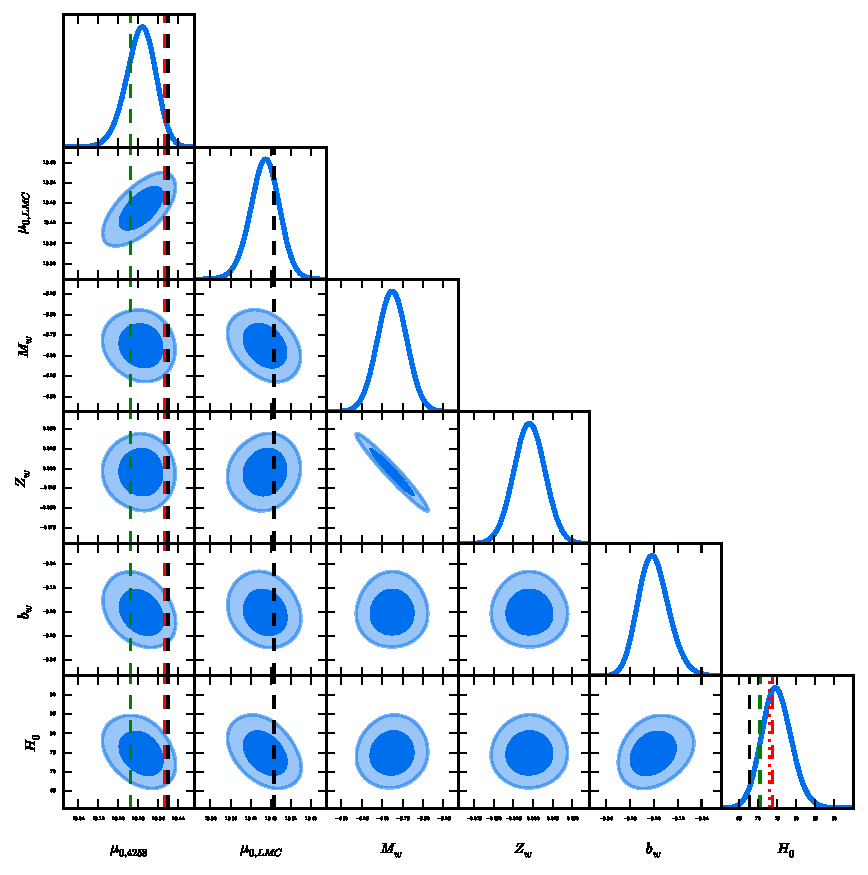
\includegraphics[scale=1]{figures/chapter-h0/triangle_plot.pdf}
\caption{Posterior constraints for fit '$M1^{a}$'. Green, red and black vertical dashed lines in $\mu_{0,4258}$ column indicates NGC 4258 distance modulus from \cite{Polshaw:2015ika}, \cite{Riess:2016jrr} and \cite{Humphreys:2013eja}, respectively. Black dashed vertical line in $\mu_{0,\LMC}$ column shows LMC distance modulus from \cite{Pietrzynski:2013gia}. Black, green, and red dashed vertical lines in $H_0$ column respectively indicate the values derived by the Planck collaboration for the base six-parameter $\Lambda$CDM model \cite{Ade:2015xua}, Efstathiou's value \cite{Efstathiou:2013via} used by Planck collaboration as a prior, and the $3\%$ measurement reported by \cite{Riess:2011yx}; The red dotted vertical line indicates the best estimate from the analysis in \cite{Riess:2016jrr}.   }
\label{Fig:Main-analysis-fitM1a}
\end{figure}

\begin{figure}[hbtp]
\centering
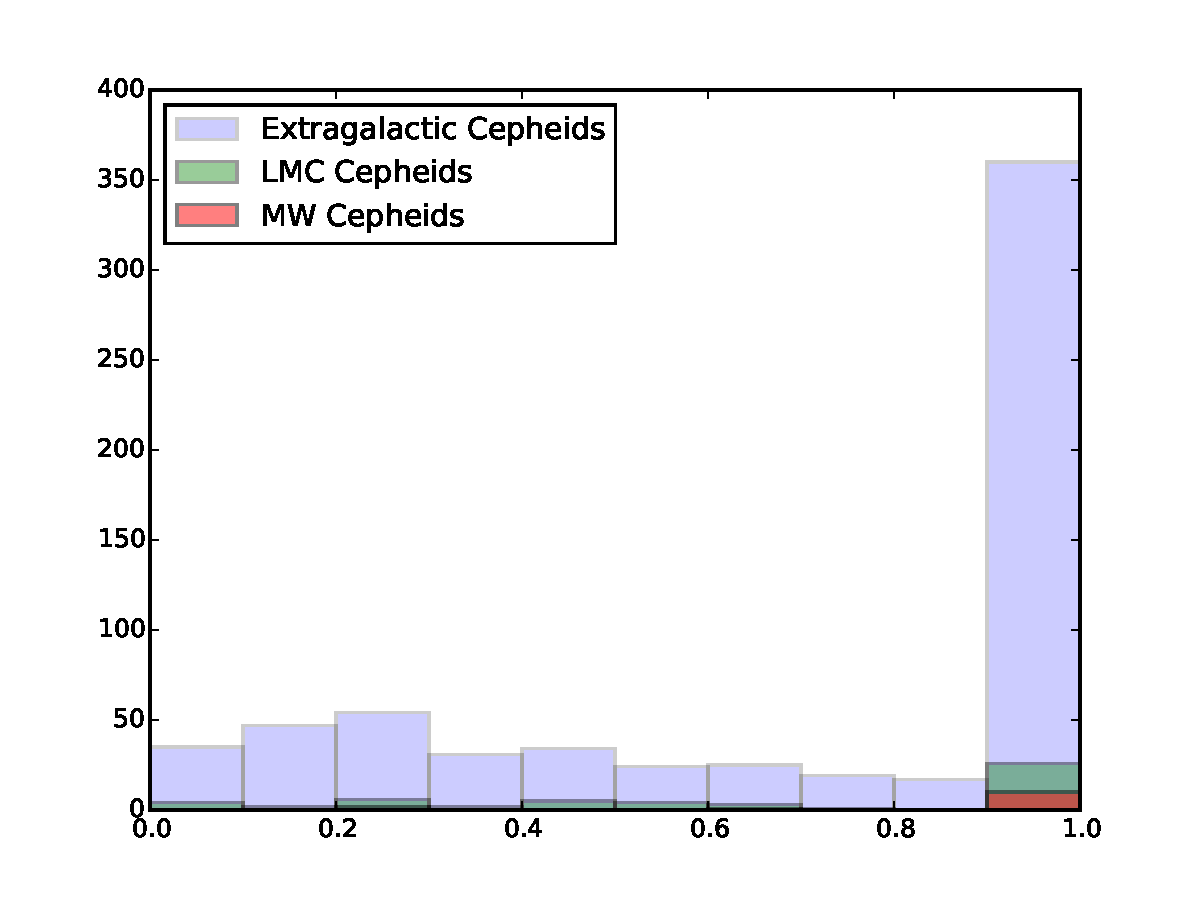
\includegraphics[scale=.75]{figures/chapter-h0/effective_HP_histogram.pdf}
\caption{Effective hyper-parameters for the sample of Cepheid variables used in fit '$M1^a$'. From the 646 Cepheid variables in the sample of \cite{Riess:2011yx}, 348 have $\alpha_{\eff}=1$, 263 $10^{-1}\leq \alpha_{\eff} < 1$, 34  $10^{-2}\leq \alpha_{\eff} < 10^{-1}$, and 1 $10^{-3} \leq \alpha_{\eff} < 10^{-2}$. For the 53 LMC Cepheid variables, the analysis outputs 25 $\alpha_{\eff}=1$, 24 $10^{-1}\leq \alpha_{\eff} < 1$, 4  $10^{-2}\leq \alpha_{\eff} < 10^{-1}$. Finally, as for the analysis shown in Figure \ref{Fig:MW-Cepheid-variables}, the set of MW Cepheid variables has 10 stars with $\alpha_{\eff}=1$ and 3 stars with $10^{-1}\leq \alpha_{\eff} < 1$. Overall, $23\%$ of the MW Cepheids are down-weighted. The fraction raises $46\%$ for Cepheids in \cite{Riess:2011yx}. As for the LMC Cepheid variables, the analysis down-weights $53\%$ of the stars.}
\label{Fig:effective-HP-fitM1a}
\end{figure}

\begin{figure}[hbtp]
\centering
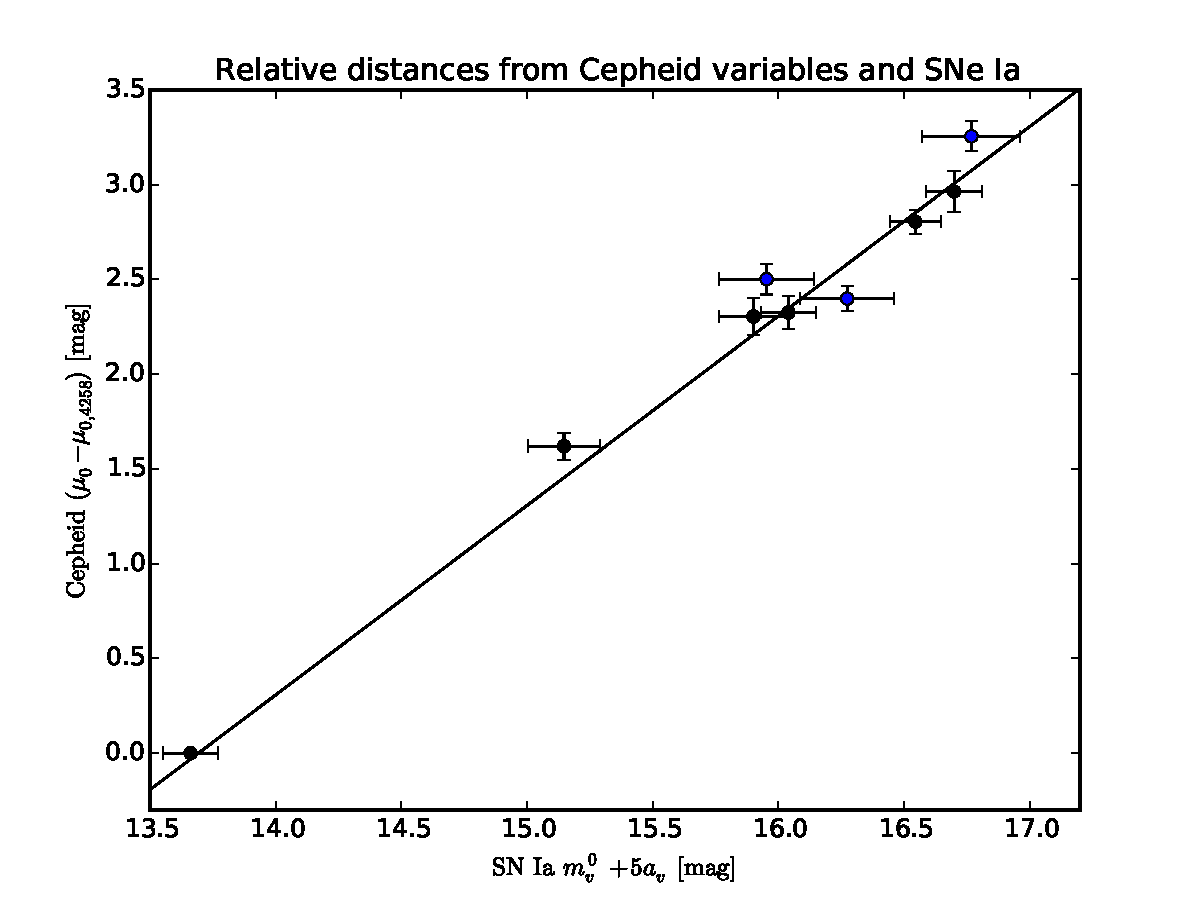
\includegraphics[scale=0.75]{figures/chapter-h0/effective_HP_SNIa.pdf}
\caption{Relative distances from Cepheids and SNe Ia. We plot the peak apparent visual magnitudes of each SN Ia (from Table 3 in \cite{Riess:2011yx}) with error bars rescaled by HP's (colour code is the same as in Figure \ref{Fig:LMC-Cepheid-variables-fit-c}) against the relative distances between hosts determined from fit '$M1^a$' in Table \ref{Table:Constraints-main-analysis}. The solid line shows the corresponding best fit. The first point on the left corresponds to the expected reddening-free, peak magnitude of an SN Ia appearing in the megamaser system NGC 4258 which is derived from the fit '$M1^a$'. }
\label{Fig:HP-SNIa-main-analysis}
\end{figure}

\begin{table}[tbp]
\centering
\begin{tabular}{@{}lccccr}
\hline
\multicolumn{6}{c}{Distance parameters} \\
\hline
Host & SN Ia & $\mu_{0,i}-\mu_{0,4258}$ & $\mu_{0,i} $ best & $\alpha_{\eff}$ & $\sigma_{\intt,i}$\\
\hline

 n4536 & SN 1981B & $1.620\,(0.071)$&$30.91\,(0.08)$ &$1$ & $0.1$ \\

 n4639 & SN 1990N & $2.325\,(0.085)$& $31.61\,(0.09)$& $1 $ & $0.03$\\

 n3370 & SN 1994ae & $2.805\,(0.063)$& $32.09\,(0.07)$& $1 $ & $0.02$ \\
 
 n3982 & SN 1998aq & $2.502\,(0.081)$& $31.79\,(0.08)$& $ 0.23$ & $0.03$\\
  
 n3021 & SN 1995al & $2.964\,(0.110)$& $32.25\,(0.11)$& $ 1$ & $0.03$\\
    
 n1309 & SN 2002fk & $3.255\,(0.079)$& $32.54\,(0.08)$& $ 0.28$ & $0.03$\\

 n5584 & SN 2007af & $2.399\,(0.064)$& $31.69\,(0.07)$& $ 0.43$ & $0.03$\\
       
 n4038 & SN 2007sr & $2.304\,(0.099)$& $31.59\,(0.11)$& $ 1$ & $0.03$\\
       
\hline
\end{tabular}
\caption{\label{Table:SNIa-HP-fit-M1a} Distance parameters for the SNe Ia hosts corresponding to our 'standard analysis'. Numbers in brackets give the standard deviation. The last two columns correspond to the effective HP for each SN Ia host and the corresponding internal scatter, respectively.}
\end{table}

These choices correspond to the case `$M1^{a}$' of Table \ref{Table:Constraints-main-analysis}. We show the parameter constraints for this case in Fig.\ \ref{Fig:Main-analysis-fitM1a}. The resulting constraint on the Hubble parameter is
\begin{equation}\label{Eq:H0-value-standard-analysis}
	H_0 = 75.0 \pm 3.9 \, \mathrm{km/s/Mpc} \, .
\end{equation}
The dashed vertical lines in the 1D marginal posterior for $H_0$ of Fig.\ \ref{Fig:Main-analysis-fitM1a} give (from left to right) the mean values of the Planck $\Lambda$CDM determination of $H_0$ ($67.8\pm0.9$ km/s/Mpc from Planck temperature and lensing data \cite{Ade:2015xua}) 
and of the analyses of \cite{Efstathiou:2013via} ($70.6\pm3.3$ km/s/Mpc), \cite{Riess:2016jrr} ($73.0\pm1.8$ km/s/Mpc), and \cite{Riess:2011yx} ($73.8\pm2.4$ km/s/Mpc). Our result here agrees best with the latter two (although our width is somewhat larger due to the use of hyper parameters), but even the Planck value lies within our $95\%$ credible interval. Note that as the HP likelihoods have wide wings and are very non-Gaussian, it could be the case that the likelihood for $H_0$ also is very
non-Gaussian. We found however that it is relatively close to a normal pdf.

Figure \ref{Fig:effective-HP-fitM1a} shows a histogram for HPs in the sample of Cepheid variables used in our 'standard analysis'. Whereas in \cite{Riess:2011yx} about $20\%$ of the Cepheids are rejected by the Chauvenet's criterion (this would be equivalent to $\alpha_{\eff}=0$ in our analysis), our analysis finds that about $46\%$ of the Cepheid variables in \cite{Riess:2011yx} are down-weighted ($\alpha_\eff <1$). The analysis in \cite{Riess:2016jrr}, also using a Chauvenet's criterion, finds an outlier fraction of $2-5\%$ in a larger sample of Cepheid variables.

Figure \ref{Fig:HP-SNIa-main-analysis} and Table \ref{Table:SNIa-HP-fit-M1a} bring about the presence of possible outliers among the sample of SNe Ia hosts, thus justifying our use of HP's in the apparent visual magnitudes of each SN Ia. This could be a hint of unaccounted systematics in the light-curve fits for those SNe Ia. Note that \cite{Riess:2016jrr} has used a different light-curve fitting algorithm (SALT-II) to that utilised in \cite{Riess:2011yx} (MLCS2k2) finding no evidence for any of their 18 SNe Ia hosts to be an outlier. 
 
As we mentioned above, the available distance modulus are included with HP's in our 'standard analysis'. The resulting effective HP's are: $\alpha^{\eff}_{\LMC}=1$, $\alpha^{\eff,\rm M1}_{\rm 4258}=0.6$, $\alpha^{\eff,\rm M2}_{\rm 4258}=1$. This shows that the geometric maser distance estimate to the active galaxy NGC 4258 from \cite{Humphreys:2013eja} is slightly down-weighted in our analysis.  As can be seen from the vertical, red, dashed line in Figure \ref{Fig:Main-analysis-fitM1a}, the revised maser distance to NGC 4258 from \cite{Riess:2016jrr} is now closer to our $68\%$ confidence region.     

Finally, we also note that it is not least the difference between the supernova distance \cite{Polshaw:2015ika} and
the maser distance \cite{Humphreys:2013eja} to NGC 4258 that limits the precision on $H_0$ as can be seen from the vertical dashed lines
for $\mu_{0,4258}$ in Fig.\ \ref{Fig:Main-analysis-fitM1a}. Especially the very recent supernova distance prefers a higher $H_0$ as can be seen
from the marginal 2D likelihood for $\mu_{0,4258}$ and $H_0$. An improvement in the anchors is thus important for future improvements in the
direct determination of the local expansion rate $H_0$. Note, however, that our 'standard analysis' is almost unaffected by the inclusion of the supernova distance \cite{Polshaw:2015ika} to the megamaser system NGC 4258. Fit '$M1^{af}$' includes only the geometric maser distance \cite{Humphreys:2013eja} and we find changes in $H_0$ and $M_W$ smaller than $0.2\%$ w.r.t our 'standard analysis'.

\subsection{Determining $H_0$ with Bayesian hyper-parameters (R16 data set)}
\label{Subsection:combining-anchors-R16}

\section{Discussion and Conclusions}
\label{chapter-h0:Summary}

%\comment{COMMENT: fig.10 to be moved before, it is our main figure. Add a table in which we fix one case (ex. M1a) and we compare different choices of the anchors. Ex. 1 line for all three, 1 line for MK, 1 line for LMC. That will be our main table. For all fits in the paper: number them from 1,2,3 on without the a,b,c indices. Then we can have 1 table with a column with the index and a line of explanation with every index: alternatively, columns corresponding to all degrees of freedom with ticks/crosses that identify what each fit is exactly doing.}

In the previous Section we presented an statistical method which allows a comprehensive treatment of the available data to determine the current expansion rate of the universe $H_0$. The use of Bayesian hyper-parameters avoids the arbitrary discard of data which is implicit in outlier rejection algorithms. Such algorithms have been used in  \cite{Riess:2009pu}, \cite{Riess:2011yx}, \cite{Efstathiou:2013via} and in some cases a dependence of the results with the statistical method utilised has been found. The determination of the Hubble constant with Bayesian hyper-parameters is robust against different assumptions in the analysis (e.g., period cut in the Cepheid variables data, prior on the metallicity parameter $Z_W$ of the period-luminosity relation) as can be seen from Table \ref{Table:Constraints-main-analysis}. In Addition, since the method utilises all the available data sets, it allows to check how consistent with each other they are and how much weight they are assigned in the fit. Low values of HPs might be due to unrecognised (or underestimated) systematics in the data sets or might be a calling for better modelling.

We have shown that, contrary to an usual $\chi^2$ approach, when Cepheid variables are fitted using HPs, the down-weighted datums (outlier candidates in an outlier rejection algorithm) do not significantly bias the slope $b_W$ in the period-luminosity relation (see Figure \ref{Fig:LMC-Cepheid-variables-fit-c} and Table \ref{Table:LMC-fits}). Note that due to degeneracies in the parameters (e.g., $H_0,\, M_W,\, b_W,\, Z_W,\,$\dots), this could also lead to bias in the determination of the Hubble constant $H_0$ in an usual $\chi^2$ analysis. Moreover, a decrement of the data set might lead to unnecessary increase of the error bars in the fitting parameters.

From Subsections \ref{Subsection:LMC}-\ref{Subsection:NGC4258} it becomes clear that the three set of Cepheid variables in the galaxies LMC, MW, and NGC 4258 are consistent with each other ($b_W$ and $M_W$ agree within error bars) thus providing no argument to exclude any of them from the main analysis. In Subsection \ref{Subsection:Zw-dependence} we have studied the period-luminosity relation of each one of the galaxies containing Cepheid variables allowing for a metallicity dependence. Table \ref{Table:Zw-dependence-of-PL-relation} shows that at least five galaxies have an slope $b_W$ which differs from that of LMC Cepheid variables by about $2\sigma$. An statistical method combining these data sets without taking those inconsistencies into account could lead to biased results (compare, for instance, $b_W$ for our fits in Appendix \ref{Section:Appendix} with those in Appendix A of \cite{Efstathiou:2013via} which are driven upwards). Our method is able to deal with those data sets thus no biasing our constraints in the period-luminosity parameters.

One of the advantages of using HPs to determine the Hubble constant is that one can assess the compatibility of the different data sets. Our 'standard analysis' includes the available Cepheid variables (i.e., no period cut), the available independent measurements of distance modulus to both NGC 4258 and LMC, and the available SNe Ia apparent magnitudes with HPs, but we have also performed several variants which are shown in Table \ref{Table:Constraints-main-analysis}. In Table \ref{Table:HPs-main-analysis-Table3} we show the HPs for the available distance modulus and the sum of effective HPs for both SNe Ia hosts and MW Cepheid variables corresponding to fits in Table \ref{Table:Constraints-main-analysis}. Fits that only differ from the 'standard analysis' either in the period cut or in the prior for the metallicity parameter $Z_W$ give consistent results: we obtain a $5\%$ measurement of $H_0 \approx 75 \pm 4\, \km\, \second^{-1}\, \Mpc^{-1}$. Differently to the 'standard analysis', the fit '$M1^{af}$' does not include the distance modulus to NGC 4258 from \cite{Polshaw:2015ika}. This change does not considerably change the constraints, but whereas MW Cepheid variables gain a bit of weight in the analysis, both SNe Ia hosts and distance modulus to NGC 4258 are more down-weighted than in the 'standard analysis'. In fact, SNe Ia hosts show the lowest degree of agreement among the different variants of fit '$M1^a$'.

In the fit '$M1^{ag}$' the value of the Hubble constant is shifted downwards by $\approx 2\%$ w.r.t. our 'standard analysis'. In this case we do not include SNe Ia hosts with HPs; This would be equivalent to assume that there are no outliers among the SNe Ia hosts assigning thus equal weight to every host galaxy in the analysis. Although this assumption both brings the distance modulus to NGC 4258 from \cite{Humphreys:2013eja} in better agreement and decreases the standard deviation in $H_0$ (it is now a $3\%$ measurement), our main analysis brings about the presence of down-weighted SNe Ia hosts (see Figure \ref{Fig:HP-SNIa-main-analysis}). Such an assumption is implicit in the analyse \cite{Riess:2011yx} and \cite{Efstathiou:2013via}. Presence of outliers among the SNe Ia hosts might be due to unaccounted (or underestimated) systematics in the light-curve fits for those SNe Ia. In \cite{Riess:2016jrr} a new, enlarged sample of $18$ SNe Ia hosts has been fitted with the SALT-II algorithm (instead of MLCS2k2 used by \cite{Riess:2011yx}) finding no evidence for outliers. Once the data becomes available, this could be easily verified with our method.

We have also studied the possibility of including the available distance modulus with equal weight in the fit, but using HPs in the SNe Ia hosts. This corresponds to the fit '$M1^{ah}$' which gives a value of $H_0$ ($5\%$ measurement) lower than in our 'standard analysis' by $\approx 1\%$. In this case the SNe Ia hosts are less down-weighted than in any other variant of fit '$M1^a$'.

In the fit '$M1^{aj}$' we have only used HPs in the Cepheid variables. This case is close to the analysis of \cite{Riess:2011yx} where they found $H_0 = 73.8 \pm 2.1 \, \km\, \second^{-1}\, \Mpc^{-1}$ the difference being the inclusion of all the available Cepheid variables (no outlier rejection applied) in fit '$M1^{aj}$'. Although the uncertainties output by the two analyses are almost the same, our $H_0$ value is lower than theirs by $\approx 2\%$. Our $H_0$ value agree better with fits $75$, $79$, and $83$ of \cite{Efstathiou:2013via} which use both period cut and outlier rejection, though.

Fit '$M1^b$' differs from '$M1^a$' in the use of a smaller subset of Cepheid variables (upper period cut of $60$ days). While the distance modulus to NGC 4258 from \cite{Humphreys:2013eja} gets down-weighted, the compatibility of the MW Cepheid variables is enhanced.

Differently to fit '$M1^b$', where we use internal scatter nuisance parameters $\sigma_{\intt}$ for each galaxy containing Cepheid variables, in fit '$M1^{be}$'  we have fixed those nuisance parameters to the values in fit $75$ of \cite{Efstathiou:2013via} and used HPs only for the Cepheid variables. The constraints output by two analyses agree within error bars; In particular, the values of $H_0$ agree pretty well. Because the role of $\sigma_{\intt}^{\MW}$ is a common increment of the error bars in the magnitudes of MW Cepheid variables, a big internal scatter $\sigma_{\intt}^{\MW}$ would mean no MW Cepheid variables down-weighted by HPs. In fit '$M1^{be}$' the internal scatter is five times greater than in fit '$M1^b$' and as a result all HPs are equal one. The use of HPs does not weaken the quality of the data as a whole, instead the method is able to identify and down-weight only those data points which are inconsistent.

In Figure \ref{Fig:H0-values-3-anchors} we show different measurements of the Hubble parameter which use three anchor distances. The precision of the measurement using HPs depends on the assumptions made as discussed above. Our 'standard analysis' and its variants agree with previous measurements \cite{Riess:2011yx} and \cite{Efstathiou:2013via} using the same data set. While analyses using HPs agree with both most recent direct local measurement of $H_0$ \cite{Riess:2016jrr} and the WMAP 2009 indirect determination \cite{Hinshaw:2012aka}, our result is in disagreement with the indirect determination by the Planck collaboration \cite{Ade:2015xua}. The fact that three different analyses converge at similar values for $H_0$ nicely shows that the result is robust. Although we have not found reasons to discard any of the data sets, in Appendix \ref{Section:Appendix} we have carried out analyses simultaneously including only one or two anchors. Those cases suggest that i) inclusion of MW Cepheid variables drives $H_0$ to higher values independently of both prior on the metallicity parameter and period cut for period-luminosity relation ii) a strong prior on the metallicity parameter when including distance modulus to LMC also drives $H_0$ to higher values. We discuss this with more details in Appendix \ref{Section:Appendix}. 

\begin{figure}[hbtp]
\centering
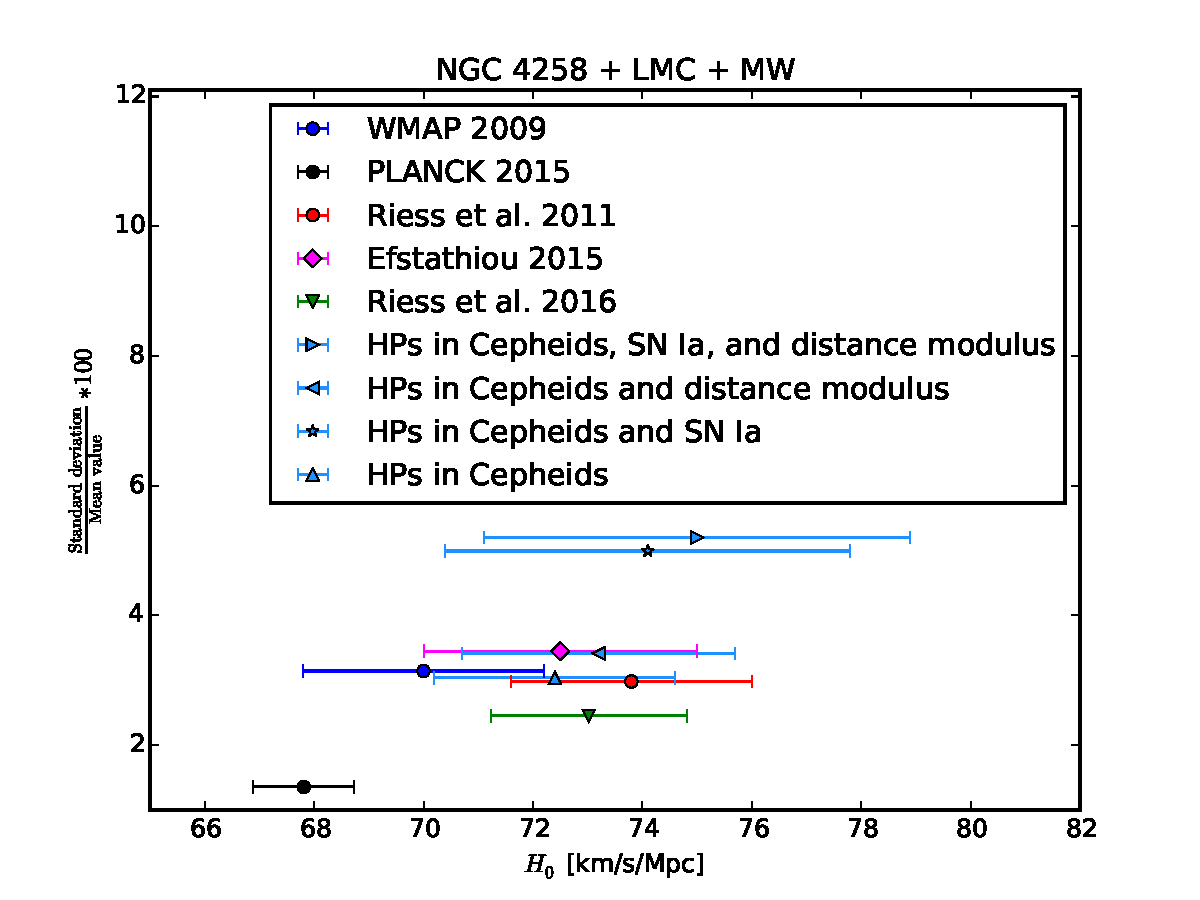
\includegraphics[scale=.75]{figures/chapter-h0/H0_values_three_anchors.pdf}
\caption{Different determinations of the Hubble constant. Blue and black show the indirect determinations by the WMAP team \cite{Hinshaw:2012aka} and by the Planck collaboration \cite{Ade:2015xua}, respectively. Direct measurements using NGC 4258 distance modulus, LMC distance modulus and MW Cepheid variables as anchor distances are shown in red, magenta, green, and dodger blue. Red corresponds to measurement by Riess et al. \cite{Riess:2011yx}, magenta shows Efstathiou's measurement \cite{Efstathiou:2013via} which uses a $60$ days period cut, green is the Riess et al. measurement \cite{Riess:2016jrr}, and dodger blue points correspond from top to bottom to fits '$M1^a$','$M1^{ag}$','$M1^{ah}$', '$M1^{aj}$' in Table \ref{Table:Constraints-main-analysis}.\label{Fig:H0-values-3-anchors}}
\end{figure}

\begin{table}[tbp]
\centering
\begin{tabular}{@{}lccccc}
\hline
\multicolumn{6}{c}{NGC $4258$ $+$ LMC $+$ MW anchors} \\
\hline
Fit & $\alpha_{4258}^{\eff,\,\rm M1}$ & $\alpha_{4258}^{\eff,\,\rm M2}$ & $\alpha_{\LMC}$ & $\sum_{i=1}^{8}  \alpha^{\eff,\,\SNe}_{i}$ &$\sum_{i=1}^{13} \alpha^{\eff,\,\MW}_{i}$ \\
\hline
$M1^{a}$ & $ 0.6 $ & $ 1 $ & $ 1 $ & $ 5.9 $ & $ 11.2 $ \\
$M1^{af}$ & $ 0.5 $ & $ $ & $ 1 $ & $ 5.4 $ & $ 11.4 $ \\
$M1^{ag}$ & $ 0.8 $ & $ 1 $ & $ 1 $ & $ $ & $ 11.1 $ \\
$M1^{ah}$ & $ $ & $ $ & $ $ & $ 6.5 $ & $ 11.5 $ \\
$M1^{aj}$ & $ $ & $ $ & $ $ & $ $ & $ 11.2 $\\
$M1^{b}$ & $ 0.3 $ & $ 1 $ & $ 1 $ & $ 5.9 $ & $ 11.9 $ \\
$M1^{be}$ & $ $ & $ $ & $ $ & $ $ & $ 13 $ \\
$M2^{a}$ & $ 0.7 $ & $ 1 $ & $ 0.4  $ & $ 6.1 $ & $ 11.2$ \\
$M2^{b}$ & $ 0.5 $ & $ 1 $ & $ 0.6 $ & $ 5.7 $ & $ 11.3 $ \\
$M3^{a}$ & $ 0.4 $ & $ 1 $ & $ 0.9 $ & $ 6.3 $ & $ 11.4 $ \\
$M3^{b}$ & $ 0.9 $ & $ 1 $ & $ 0.2 $ & $ 6.0 $ & $ 11.0 $ \\
%$M3^{a}$ & $75.0\,(3.9)$ & $-5.92\,(0.04)$ & $-3.20\,(0.05)\,[N]$ & $0$ & $0.06$ & $0.02$ \\
%$M3^{b}$ & $75.4\,(3.7)$ & $-5.92\,(0.04)$ & $-3.27\,(0.04)\,[N]$ & $ 0 $ & $0.06$ & $0.02$ \\
\hline
\end{tabular}
\caption{\label{Table:HPs-main-analysis-Table3} Effective hyper-parameters for distance modulus used in fits of Table \ref{Table:Constraints-main-analysis} and the sum of effective HPs for both SNe Ia hosts and MW Cepheid variables.%\comment{COMMENT: reminder, change labels M1, M2, renormalise last two columns to 1}}
}
\end{table}